%% For double-blind review submission, w/o CCS and ACM Reference (max submission space)
\documentclass[sigplan,10pt,review,anonymous]{acmart}\settopmatter{printfolios=false,printccs=false,printacmref=false}
\settopmatter{printacmref=false} % Removes citation information below abstract
\renewcommand\footnotetextcopyrightpermission[1]{} % removes footnote with conference information in first column
\pagestyle{plain} % removes running headers

%% For double-blind review submission, w/ CCS and ACM Reference
%\documentclass[sigplan,review,anonymous]{acmart}\settopmatter{printfolios=true}
%% For single-blind review submission, w/o CCS and ACM Reference (max submission space)
%\documentclass[sigplan,review]{acmart}\settopmatter{printfolios=true,printccs=false,printacmref=false}
%% For single-blind review submission, w/ CCS and ACM Reference
%\documentclass[sigplan,review]{acmart}\settopmatter{printfolios=true}
%% For final camera-ready submission, w/ required CCS and ACM Reference
%\documentclass[sigplan]{acmart}\settopmatter{}


%% Conference information
%% Supplied to authors by publisher for camera-ready submission;
%% use defaults for review submission.
% \acmConference[PL'18]{ACM SIGPLAN Conference on Programming Languages}{January 01--03, 2018}{New York, NY, USA}
% \acmYear{2018}
% \acmISBN{} % \acmISBN{978-x-xxxx-xxxx-x/YY/MM}
% \acmDOI{} % \acmDOI{10.1145/nnnnnnn.nnnnnnn}
\startPage{1}

%% Copyright information
%% Supplied to authors (based on authors' rights management selection;
%% see authors.acm.org) by publisher for camera-ready submission;
%% use 'none' for review submission.
\setcopyright{none}
%\setcopyright{acmcopyright}
%\setcopyright{acmlicensed}
%\setcopyright{rightsretained}
%\copyrightyear{2018}           %% If different from \acmYear

%% Bibliography style
\bibliographystyle{ACM-Reference-Format}
%% Citation style
%\citestyle{acmauthoryear}  %% For author/year citations
%\citestyle{acmnumeric}     %% For numeric citations
%\setcitestyle{nosort}      %% With 'acmnumeric', to disable automatic
                            %% sorting of references within a single citation;
                            %% e.g., \cite{Smith99,Carpenter05,Baker12}
                            %% rendered as [14,5,2] rather than [2,5,14].
%\setcitesyle{nocompress}   %% With 'acmnumeric', to disable automatic
                            %% compression of sequential references within a
                            %% single citation;
                            %% e.g., \cite{Baker12,Baker14,Baker16}
                            %% rendered as [2,3,4] rather than [2-4].


%%%%%%%%%%%%%%%%%%%%%%%%%%%%%%%%%%%%%%%%%%%%%%%%%%%%%%%%%%%%%%%%%%%%%%
%% Note: Authors migrating a paper from traditional SIGPLAN
%% proceedings format to PACMPL format must update the
%% '\documentclass' and topmatter commands above; see
%% 'acmart-pacmpl-template.tex'.
%%%%%%%%%%%%%%%%%%%%%%%%%%%%%%%%%%%%%%%%%%%%%%%%%%%%%%%%%%%%%%%%%%%%%%

%% Other packages
\usepackage{algorithm}
\usepackage[noend]{algpseudocode}
\usepackage{algorithmicx}
\usepackage{tikz}
\usetikzlibrary{positioning,shadows,arrows,trees,shapes,fit}
\usepackage{pgfplots}
\pgfplotsset{compat=1.12}
\usepackage{pgfplotstable}
\usepackage{bm}
\usepackage{framed}
\usepackage{amsmath}
\usepackage{amssymb}
\usepackage{xspace}
\usepackage{listings}

\lstset{
  language=Caml,
  basicstyle=\ttfamily,
  keywordstyle=\ttfamily,
}

\lstnewenvironment{code}{
\lstset{
  language=Caml,
  basicstyle=\ttfamily,
  keywordstyle=\ttfamily,
}}
{}

\lstnewenvironment{ecode}{
\lstset{
  language=Caml,
  basicstyle=\small\ttfamily,
  keywordstyle=\ttfamily\bfseries,
  numbers=left,
  xleftmargin=5.5mm,
  moredelim=[is][\bfseries]{==}{==},
  moredelim=[is][\underbar]{__}{__},
  moredelim=[is][\bfseries\underbar]{_=}{=_},
  escapeinside={(*@}{@*)}
}}
{}

\lstnewenvironment{compactcode}{
\lstset{
  language=Caml,
  basicstyle=\small\ttfamily,
  keywordstyle=\ttfamily\bfseries,
  xleftmargin=0mm,
  moredelim=[is][\bfseries]{==}{==},
  moredelim=[is][\underbar]{__}{__},
  moredelim=[is][\bfseries\underbar]{_=}{=_},
  escapeinside={(*@}{@*)}
}}
{}

\lstnewenvironment{haskellcode}{
\lstset{
  language=haskell,
  basicstyle=\small\ttfamily,
  keywordstyle=\ttfamily\bfseries,
  moredelim=[is][\bfseries]{==}{==},
  moredelim=[is][\underbar]{__}{__},
  moredelim=[is][\bfseries\underbar]{_=}{=_},
  escapeinside={(*@}{@*)}
}}
{}

\MakeRobust{\Call}

\newcommand{\algorithmautorefname}{Algorithm}

\lstMakeShortInline[mathescape=true]{|}

%% Our commands
\usepackage{commands}

%% Some recommended packages.
\usepackage{booktabs}   %% For formal tables:
                        %% http://ctan.org/pkg/booktabs
\usepackage{subcaption} %% For complex figures with subfigures/subcaptions
                        %% http://ctan.org/pkg/subcaption


\begin{document}

%% Title information
% \title[\toolname]{\toolname: Repairing Incorrect \\ Programming Assignment Solutions}
\title[\toolname]{Error Feedback via Analytic Program Repair}
% \titlenote{with title note}             %% \titlenote is optional;
%                                         %% can be repeated if necessary;
%                                         %% contents suppressed with 'anonymous'
% \subtitle{Subtitle}                     %% \subtitle is optional
% \subtitlenote{with subtitle note}       %% \subtitlenote is optional;
%                                         %% can be repeated if necessary;
%                                         %% contents suppressed with 'anonymous'
%% Author information
%% Contents and number of authors suppressed with 'anonymous'.
%% Each author should be introduced by \author, followed by
%% \authornote (optional), \orcid (optional), \affiliation, and
%% \email.
%% An author may have multiple affiliations and/or emails; repeat the
%% appropriate command.
%% Many elements are not rendered, but should be provided for metadata
%% extraction tools.

%% Author with single affiliation.
\author{First1 Last1}
\authornote{with author1 note}          %% \authornote is optional;
                                        %% can be repeated if necessary
\orcid{nnnn-nnnn-nnnn-nnnn}             %% \orcid is optional
\affiliation{
  \position{Position1}
  \department{Department1}              %% \department is recommended
  \institution{Institution1}            %% \institution is required
  \streetaddress{Street1 Address1}
  \city{City1}
  \state{State1}
  \postcode{Post-Code1}
  \country{Country1}                    %% \country is recommended
}
\email{first1.last1@inst1.edu}          %% \email is recommended

%% Author with two affiliations and emails.
\author{First2 Last2}
\authornote{with author2 note}          %% \authornote is optional;
                                        %% can be repeated if necessary
\orcid{nnnn-nnnn-nnnn-nnnn}             %% \orcid is optional
\affiliation{
  \position{Position2a}
  \department{Department2a}             %% \department is recommended
  \institution{Institution2a}           %% \institution is required
  \streetaddress{Street2a Address2a}
  \city{City2a}
  \state{State2a}
  \postcode{Post-Code2a}
  \country{Country2a}                   %% \country is recommended
}
\email{first2.last2@inst2a.com}         %% \email is recommended
\affiliation{
  \position{Position2b}
  \department{Department2b}             %% \department is recommended
  \institution{Institution2b}           %% \institution is required
  \streetaddress{Street3b Address2b}
  \city{City2b}
  \state{State2b}
  \postcode{Post-Code2b}
  \country{Country2b}                   %% \country is recommended
}
\email{first2.last2@inst2b.org}         %% \email is recommended


%% Abstract
%% Note: \begin{abstract}...\end{abstract} environment must come
%% before \maketitle command
\begin{abstract}
Text of abstract \ldots.
\end{abstract}


%% 2012 ACM Computing Classification System (CSS) concepts
%% Generate at 'http://dl.acm.org/ccs/ccs.cfm'.
\begin{CCSXML}
<ccs2012>
<concept>
<concept_id>10011007.10011006.10011008</concept_id>
<concept_desc>Software and its engineering~General programming languages</concept_desc>
<concept_significance>500</concept_significance>
</concept>
<concept>
<concept_id>10003456.10003457.10003521.10003525</concept_id>
<concept_desc>Social and professional topics~History of programming languages</concept_desc>
<concept_significance>300</concept_significance>
</concept>
</ccs2012>
\end{CCSXML}

\ccsdesc[500]{Software and its engineering~General programming languages}
\ccsdesc[300]{Social and professional topics~History of programming languages}
%% End of generated code


%% Keywords
%% comma separated list
\keywords{keyword1, keyword2, keyword3}  %% \keywords are mandatory in final camera-ready submission


%% \maketitle
%% Note: \maketitle command must come after title commands, author
%% commands, abstract environment, Computing Classification System
%% environment and commands, and keywords command.
\maketitle

\section{Introduction}
\label{sec:intro}

% The problem
%
Languages with Hindley-Milner style, unification-based inference
offer the benefits of static typing with minimal annotation overhead.
The catch, however, is that programmers must first ascend the steep
learning curve associated with understanding the \emph{error messages}
produced by the compiler.
%
While \emph{experts} can, usually, readily decipher the errors, and
view them as invaluable aids to program development and refactoring,
\emph{novices} are typically left quite befuddled and frustrated,
without a clear idea of \emph{what} the problem is~\citep{Wand1986-nw}.
%
Owing to the importance of the problem, several authors have proposed methods to
help debug type errors, typically, by \emph{slicing} down the program to the
problematic locations~\citep{Haack2003-vc, Rahli2015-tt}, by \emph{enumerating}
possible causes \citep{Lerner2007-dt, Chen2014-gd}, or by \emph{ranking} the
possible locations using MAX-SAT
\citep{Pavlinovic2014-mr}, Bayesian~\citep{Zhang2014-lv}
or statistical analysis~\citep{Seidel:2017}.
%
While valuable, these approaches at best help localize
the problem but students are still left in the dark
about how to \emph{fix} their code.

% Repairs as error messages?
\mypara{Repairs as Feedback}
%
Several recent papers have proposed an inspiring new line of
attack on the feedback problem: using techniques from synthesis
to provide feedback in the form of \emph{repairs} that students
can apply to improve their code.
%
These repairs are found either by symbolically searching a space of candidate
programs circumscribed by an expert-defined repair model
\citep{singh2013,HeadGSSFDH17}, or via the observation that \emph{similar
programs} have similar repairs, \ie by calculating ``diffs'' from the given
solution and a \emph{correct} program that is the ``closest'' to the student's
solution ~\citep{Gulwani_2018,Wang_2018}

While this approach is compelling for generating feedback in large
classes, it has several crucial requirements that render it inapplicable
for type error messages.
%
First, for type errors, the space of candidate repairs is massive.
It is quite unclear whether a small set of repair models \emph{exists}
or even if it does, what it \emph{looks like}. More importantly,
to scale, it is essential that we remove the requirement that an
expert carefully curate some set of candidate repairs.
%
Second, the approach requires a corpus of similar programs,
whose syntax trees or execution traces can be used to match
each incorrect program with a ``correct'' version that is
used to provide feedback. Programs with static type errors
have no execution traces.
%
More importantly, we desire a means to generate feedback
for \emph{new} programs that novices write, and hence
cannot rely on matching against some (existing) correct
program.

\mypara{Analytic Program Repair}
%
In this work, we present a novel error repair
strategy called \emph{Analytic Program Repair}
that uses supervised learning instead of manually
crafted repair models or matching against a corpus
of correct code.
%
Our strategy is based on the key insight that
\emph{similar errors} have similar repairs.
%
Our strategy realizes the above insight by using
a training dataset of pairs of ill-typed programs
and their fixed versions to:
%
(1)~\emph{learn} a collection of candidate repair templates
    by abstracting and partitioning the edits made in the
    training set into a representative set of templates;
%
(2)~\emph{predict} the appropriate template from a given error,
    by training multi-class classifiers on the repair templates
    used in the training set;
%
(3)~\emph{synthesize} a concrete repair from the template
   by enumerating and ranking correct (\eg well-typed)
   terms matching the predicted template,
%
thereby, generating a fix from a candidate program.
%
Critically, we show how to perform the crucial abstraction
from a particular \emph{program} to an abstract \emph{error}
by representing programs via \emph{bag-of-abstracted-terms} (BOAT)
\ie as numeric vectors of syntactic and semantic features \citep{Seidel2017-ko}.
%
This abstraction lets us train predictors over high-level
code features, \ie to learn correlations between features
that cause errors and their corresponding repairs, allowing
the analytic approach to generalize beyond matching against
existing programs.

\mypara{\toolname}
%
We have implemented our approach in \toolname: a type error reporting
tool for \ocaml programs. We train (and evaluate) \toolname on a set of
over 4,500 ill-typed \ocaml programs drawn from two years of an
introductory programming course.
%
Given a new ill-typed program, \toolname generates a list of potential
solutions ranked by likelihood and an \emph{edit-distance} metric.
We train \toolname on programs from one year and evaluate in several
ways.
%
First, we measure its \emph{accuracy}: we show that \toolname correctly
predicts the right repair template {FIXME} times.
%
Second, we measure its \emph{efficiency}: we show that \toolname is able
to synthesize a concrete repair {FIXME} of the time in XXX seconds.
%
Finally, we measure the \emph{quality} of the generated messages via
a user study with 29 participants and show that
humans perceive both \toolname's edit locations and final repair quality
to be better than those produced by \seminal, a state-of-the-art OCaml
repair tool \citep{Lerner2007-dt} in a statistically-significant manner.
%
This improvement shown by our data-driven method is especially
significant because \seminal incorporates several expert-guided
heuristics for improving the quality of error messages by biasing
its reports towards simpler and more useful ones.
%
Thus, our results demonstrate that data can be an 
% WRW thinks this is an odd word choice: unreasonably
effective tool in the quest for better error messages.


% First, what is a repair and when are two repairs similar?
% Second, what is an error and when are two errors similar?
% Third, how do we automatically match (similar) errors to (similar) repairs?
%
% \mypara{Repairs}
% \mypara{Errors}
% \mypara{Predicting Repairs from Errors}
% \tool converts this insight into an error reporting algorithm by addressing three crucial questions.
%%* How to \emph{curate} a collection of generic repairs?
%%* How to \emph{predict} which generic repair applies to a given error?
%%* How to \emph{synthesize} a concrete repair that fixes the given error?
%%
%%
%%We must address two crucial quie
%%To make this insight actionable, we
%%To convert this insight into an er
%%That is, rather than associating errors and repo
%%
%%
%%generalizes the key observation
%%
%%that is inspired by the synthesis approaches, but generalizes their
%%
%%Inspired by the above,
%%
%%
%%% Our approach
%%- RITE:
    %%1. repairs? learn family of repair-templates from student dataset (generalizable, fine-grained edits, not whole program)
    %%2. similar? train multi-labeled classifiers on BOAT; given new program predict location+template
    %%3. message? enumerative synthesis to fill in template at location using type-checker as oracle.

\section{Overview}
\label{sec:overview}

We begin with an overview of our approach to suggesting fixes for various faulty
programs by collectively learning from the processes novice programmers follow
to fix errors in their programs.

\begin{figure}[ht]
\begin{ecode}
let rec mulByDigit i l =
  match l with
  | []     -> []
  | hd::tl -> (hd * i) @ mulByDigit i tl
\end{ecode}

\begin{ecode}
let rec mulByDigit i l =
  match l with
  | []     -> []
  | hd::tl -> [hd * i] @ mulByDigit i tl
\end{ecode}
\caption{(top) An ill-typed \ocaml program that should multiply each element
of a list by an integer. (bottom) The fixed version by the student.}
\label{fig:mulByDigit}
\end{figure}


\mypara{The Problem.} Consider the program \mbd shown at the top of
\autoref{fig:mulByDigit}, written by a student in an undergraduate Programming
course. The program is meant to multiply all the numbers in a list with an
integer digit. The student accidentally misuses the list append operator
(\texttt{@}), applying it to a number and a list rather than two lists.
%
Novice students who are still building a mental model of how the type checker
works are often perplexed by the compiler's error message \citep{Munson_2016}.
Hence a novice will often take a long time to arrive at a suitable fix, such as
the one shown at the bottom of \autoref{fig:mulByDigit}, where \texttt{@} is
used with a singleton list containing the multiplication of the head \texttt{hd}
and \texttt{i}.
%
Our goal is to use historical data of how programmers have fixed similar errors
in their programs to automatically and rapidly guide novices to come up with
candidate solutions like the one above.


\mypara{Solution: Analytic Program Repair.}
%
One approach is to view the search for candidate repairs
as a synthesis problem: synthesize a (small) set of edits
to the program that yields a good (\eg type-correct) one.
%
To ensure that synthesis is tractable, the search must be
carefully restricted to a relatively small, manually-constructed
``repair model'' that may not include the ``right'' fixes for
an erroneous program.
%FIXME: We are not manually constructing the repair model? I might make this
% sentence more clear
%
In this work, we present a novel strategy called
\emph{Analytic Program Repair} which breaks the
problem into three parts:
%
First, \emph{learn} a set of widely used \emph{fix templates}.
%
Second, \emph{predict}, for each erroneous program, the correct fix template to apply.
%
Third, \emph{synthesize} candidate repairs from the predicted template.

In the remainder of this section, we give a high-level overview
of our approach by describing how to:

\begin{enumerate}

  \item Represent fixes abstractly via \emph{fix templates}
        (\S~\ref{sec:overview:templates}),

  \item Acquire a \emph{training set} of labeled ill-typed programs and fixes
        (\S~\ref{sec:overview:data}),

  \item Learn a small set of candidate fix templates by \emph{partitioning}
        the training set (\S~\ref{sec:overview:learn}),

  \item Predict the appropriate template to apply by training a
        \emph{multi-class classifier} from the training set
        (\S~\ref{sec:overview:predict}), and

  \item Synthesize fixes by enumerating and checking terms from the
        predicted templates to give the programmer localized feedback
        (\S~\ref{sec:overview:synthesis}).
\end{enumerate}

\subsection{Representing Fixes}
\label{sec:overview:templates}

Our notion of a fix is defined as a \emph{replacement} of an existing expression
with a new \emph{candidate} expression at a specific program location. For
example, the \mbd program is fixed by replacing |(hd * i)| with the candidate
expression |[hd * i]| on line 4. We focus on AST-level replacements as they are
compact yet expressive enough to represent fixes.


\mypara{Generic Abstract Syntax Trees.}
%
We represent the different possible candidate expressions via abstract fix
templates called \emph{Generic Abstract Syntax Trees} (GAST) which each
corresponds to many possible candidate expressions.
%
GASTs are obtained from concrete ASTs in two steps.
%
First, we abstract concrete variable, function, and operator names.
%
Next, we prune GASTs at a certain depth $d$ to keep only the top-level changes
of the fix. Pruned sub-trees are replaced with \emph{holes}, which can represent
\emph{any} possible expression in our language.


Together, these steps ensure that GASTs only contain information about a fix's
\emph{structure} rather than the specific changes in variables and functions.
%
For example, the fix |[hd * i]| in the \mbd example would be represented by the
GAST of the expression |[_ $\oplus$ _]|, where variables |hd| and |i| are
abstracted into holes (\eg by pruning the GAST at a depth $d=2$) and |*| is
represented by an abstract binary operator. Our GAST approach is similar to
that of Lerner \emph{et al.}~\citep{Lerner2007-dt}, where AST-level modifications are used, but our proposed
GASTs will represent more abstract fix schemas.


\subsection{Acquiring a Fix-Labeled Training Set}
\label{sec:overview:data}

Previous work has used experts to create a set of ill-typed programs and their
fixed versions~\citep[][]{Lerner2007-dt, Loncaric2016-uk}, or to manually create
\emph{fix templates}~\cite{kim13par} that can yield \emph{repair
patches}~\citep[][]{martinez2013automatically,martinez2015mining}.
%
These approaches are hard to scale up to yield datasets suitable for machine
learning. Also, they do not discover the \emph{frequency} in practice of particular
classes of novice mistakes and their fixes.
%
In contrast, we show that such fix templates can be \emph{learned} from a large,
automatically constructed training set of ill-typed programs labeled with their
repairs.
%
Fixes in our dataset are represented as the ASTs of the expressions that students
changed in the ill-typed program to transform it into the correct solution.

\mypara{Interaction Traces.}
Following Seidel and Jhala~\citep{Seidel:2017}, we extract a labeled
dataset of erroneous programs
and their fixed versions from \emph{interaction traces}. Usually students write
several versions of their programs until they reach the correct solution for a
programming assignment. An instrumented compiler is used to capture such
sequences (or \emph{traces}) of student programs. The first type-correct
solution in this sequence of attempts is considered to be the fixed
version of all the previous ones and thus a pair for each of them is added to
the dataset. For each program pair, we then produce a \emph{diff} of their
abstract syntax trees (ASTs), and assign as the dataset's fix labels the
\emph{smallest} sub-tree that changed between the correct and ill-typed attempt
of the program.


\subsection{Learning Candidate Fix Templates}
\label{sec:overview:learn}

Each labeled program in our dataset contains a fix, which we abstract to a fix
template. For example, in the \mbd program from \autoref{fig:mulByDigit} we get
the fix candidate |[hd * i]| and hence the fix template |[_ $\oplus$ _]|.
However, a large dataset of fix-labeled programs, which may include many
diverse solutions, can introduce a huge set of fix templates, which can be
inappropriate for predicting the correct one to be used for the final program
repair.

Therefore, the next step in our approach is to learn a set of fix templates
that is \emph{small enough} to automatically predict which template to apply to
a given erroneous program, but nevertheless \emph{covers} most of the fixes that
arise in practice.

\mypara{Partitioning the Fixes.} We learn a suitable small set of fix
templates by \emph{partitioning} all the templates obtained from our dataset,
and then selecting a single GAST to represent the fix templates from each fix
template set.
%
The partitioning serves two purposes.
%
First, it identifies a small set of the most common fix templates which then
enables the use of discrete classification algorithms to predict which template
to apply to a new program.
%
Second, it allows for the principled removal of outliers that arise because
student submissions often contain non-standard or idiosyncratic solutions that
we do not wish to use for suggesting fixes.

Unlike previous repair approaches that have used clustering to group together
similar programs (e.g.,~\citep{Wang_2018, Gulwani_2018}), we partition our set of
fix templates into their \emph{equivalence classes} based on a fix similarity
relation.


\subsection{Predicting Templates via Multi-class Classification}
\label{sec:overview:predict}

Next, we train models that can correctly predict error locations and fix
templates for a given ill-typed program. We use these models to generate
candidate expressions as possible program fixes. To reduce the
complexity of predicting the correct fix templates and error locations, we
separate these problems and encode them into two distinct \emph{supervised
classification} problems.

\mypara{Supervised Multi-Class Classification.}
We propose using a \emph{supervised multi-class classification} problem for
predicting fix templates. A \emph{supervised} learning problem is one where,
given a labeled training set, the task is to learn a function that accurately
maps the inputs to output labels and generalizes to future inputs. In a
\emph{classification} problem, the function we are trying to learn maps inputs
to a discrete set of two or more output labels, called \emph{classes}.
Therefore, we encode the task of learning a function that will map
subexpressions of ill-typed programs to a small set of fix templates as a
\emph{multi-class} classification (MCC) problem.

\mypara{Feature Extraction.} The machine learning models that we will train
to solve our MCC problem expect datasets of labeled \emph{fixed-length vectors}
as inputs. Therefore, we define a transformation of fix-labeled programs to
fixed-length vectors. Similarly to Seidel \emph{et al.}~\citep{Seidel:2017}, we define a set of
feature extraction functions $f_1, \ldots, f_n$, that map program subexpressions
to a numeric value (or just $\{0, 1\}$ to encode a boolean property). Given a
set of feature extraction functions, we can represent a single program's AST as
a set of fixed-length vectors by decomposing the AST $e$ into a set of its
constituent subexpressions $\{e_1, \ldots, e_m\}$ and then representing each
$e_i$ with the $n$-dimensional vector $[f_1(e_i), \ldots, f_n(e_i)]$. This
method is known as a \emph{bag-of-abstracted-terms} (BOAT) representation in
previous work. % FIXME: CITE

\mypara{Predicting Templates via MCC.}
Our fix-labeled dataset can be updated so the labels represent the corresponding
template that fixes each location, drawn from the minimal set of fix templates
that were acquired through partitioning. We then train a \emph{Deep Neural
Network (DNN)} classifier on the updated template-labeled data set.

Neural networks have the advantage of associating each class with a
\emph{confidence score} that can be interpreted as the model's confidence of
each class being correct for a given input. This confidence score can be used to
rank fix-template predictions for new programs and use them in descending order
to synthesize repairs until our high-level goal is reached. %FIXME: I might respecify this goal
Exploiting recent advances in machine learning, we use deep and dense
architectures \citep{Schmidhuber_2015} for more accurate fix template predictions.

\mypara{Error Localization.} We view the problem of finding error locations
in a new program as a \emph{binary} classification problem. In contrast with the
template prediction problem, we want to learn a function that maps a program's
subexpressions to a binary output representing the presence of an error or not.
Therefore, this problem is a equivalent to a MCC with only two classes and thus,
we use similar deep architectures of neural networks. For each expression in a
given program, the learned model outputs a confidence score representing how
likely it is an error location that needs to be fixed. We exploit those scores
to synthesize candidate expressions for each location in descending order of
confidence.
% We use this approach, rather than standard fault localization, because FIXME.

\subsection{Synthesizing Feedback from Templates}
\label{sec:overview:synthesis}

Next, we utilize existing program synthesis techniques to \emph{synthesize}
candidate expressions that will be used to provide feedback to users.
Guided by our learned fix-template predictions and a set of
possible error locations to guide program synthesis, we return a ranked
list of \emph{minimal} repairs to users as feedback.

\mypara{Program Synthesis.} Given a set of locations and candidate templates for
those locations, we are trying to solve a problem of \emph{program synthesis}.
For each program location, we search over all possible
expressions in the language's grammar for a small set of candidate
expressions that match the fix template and make the program type-check.
Expressions from the ill-typed program are also used during synthesis
to prune the search space of candidate expressions.

\mypara{Synthesis for Multiple Locations.}
It is often the case that more than one location needs to be fixed. Therefore,
we do not only consider the ordered set of single error locations for synthesis,
but rather its power set. For simplicity, we consider fixing different program
locations as independent; the probability we assign that a set of locations
needs to be fixed is thus the product their individual confidence scores. This
is unlike recent approaches to multi-hunk program repair~\citep{Saha_2019}
where modifications depend on each other.

\mypara{Ranking Fixes.} Finally, we rank each solution by two metrics, the
\emph{tree-edit distance} and the \emph{string-edit} distance. Previous work
\citep{Lerner2007-dt, Wang_2018, Gulwani_2018} has used such metrics to consider
minimal changes, \ie changes that are as close as possible to the original
programs, so novice programmers are presented with more coherent feedback.
% Additionally, more experienced programmers might have in mind what \emph{type}
% they want their functions to be. We thus provide the user with the option to
% give the intended type for the program's functions we are trying to repair. In
% our evaluation, we acquire the intended types from the fixed versions of the
% dataset (see \autoref{sec:synthesis}).

\begin{figure}[ht]
  \begin{ecode}
  let rec mulByDigit i l =
    match l with
    | []     -> []
    | hd::tl -> [(*@$v_1$@*) * (*@$v_2$@*)] @ mulByDigit i tl
  \end{ecode}
  \caption{A candidate repair for the \mbd program.}
  \label{fig:repair}
  \end{figure}

\mypara{Example.} We see in \autoref{fig:repair} a minimal repair that our
method could return (|[$v_1$ * $v_2$]| in line 4), using the template discussed
in \S~\ref{sec:overview:learn} to synthesize this solution. While this solution
is not the highest-ranked that our implementation returns (which would be
identical to the human solution), it demonstrates relevant aspects of the
synthesizer. In particular, this solution has some abstracted variables, $v_1$
and $v_2$. Our algorithm suggests to the user that they can replace the two
variables with two distinct variables and insert the whole expression into a
list, in order to obtain the correct program. We hypothesize that such solutions
produced by our algorithm can provide valuable feedback to novices, and we
investigate that claim empirically in \S~\ref{sec:eval:useful}.

\section{Learning Fix Templates}
\label{sec:templ-partition}

We start by introducing our approach for extracting useful \emph{fix templates}
from a training dataset comprised of paired erroneous and fixed programs.
%
We express those templates in terms of a language that allows us to succinctly
represent fixes in a way that captures the essential structure of various fix
patterns that novices use in practice.
%
However, extracting a single fix template for \emph{each} fix in the program
pair dataset yields too many templates to perform accurate predictions.
%
Hence, we define a \emph{similarity} relation between templates, which we use to
\emph{partition} the extracted templates into a smaller set, that will make it
easier to train precise models to predict fixes.

\begin{figure}
\small
\centering
\begin{minipage}[c]{\linewidth}
  \[
  \boxed{
  \begin{array}{rcl}
  e & ::=    & x \spmid \efun{x}{e} \spmid \eapp{e}{e} \spmid \elet{x}{e}{e} \\
    & \spmid & n \spmid \eplus{e}{e}\\
    & \spmid & b \spmid \eif{e}{e}{e} \\
    & \spmid & \epair{e}{e} \spmid \epcase{e}{x}{x}{e} \\
    & \spmid & \enil \spmid \econs{e}{e} \spmid \ecase{e}{e}{x}{x}{e} \\[0.05in]

  n & ::= &  0, 1, -1, \ldots \\[0.05in]

  b & ::= &  \etrue \spmid \efalse \\[0.05in]

  t & ::= & \alpha \spmid \tbool \spmid \tint \spmid \tfun{t}{t} \spmid \tprod{t}{t} \spmid \tlist{t} \\[0.05in]
  \end{array}
  }
  \]
  \captionof{figure}{Syntax of \repairLang}
  \label{fig:syntax}
\end{minipage}
\begin{minipage}[c]{\linewidth}
  \lstDeleteShortInline{|} % sigh...
  \[
  \boxed{
  \begin{array}{lcl}
    \V           & \defeq & \List{\R}\\
    \Runit       & \defeq & \{r \in \R\ |\ 0 \le r \le 1\} \\ % [0,1]\\
    \T           & \defeq & e\\
    \featuresym  & : & \List{e \to \R} \\
    \labelsym    & : & e \times e \to \List{e} \\
    \extractTsym & : & \featuresym \to e \times e \to \List{\V \times \List{\T}} \\
    \trainTsym   & : & \List{\V \times \List{\T}} \to \Model \\
    \predictTsym & : & \Model \to \V \to \List{\Runit} \\
    \midrule
    \repairsym   & : & \Model \to e \to \List{e \times \Runit \times \List{\Runit}}
  \end{array}
  }
  \]
  \lstMakeShortInline{|}
  \captionof{figure}{
    A high-level API for converting program pairs to
    feature vectors and template labels.
  }
  \label{fig:api}
\end{minipage}
\end{figure}


\subsection{Representing User Fixes}
\label{sec:templ-partition:lang}

\mypara{Repair Template Language.}
\autoref{fig:rtl-syntax} describes our Repair Template Language, \repairLang,
which is a lambda calculus with integers, booleans, pairs, and lists, that
extends our core ML language \lang (\autoref{fig:ml-syntax}) with
syntactic abstraction forms:

\begin{enumerate}
    \item \emph{Abstract variable} names $\hat{x}$  are used to denote variable
    occurrences for functions, variables and binders, \ie $\hat{x}$ denotes
    an unknown variable name in \repairLang;

    \item \emph{Abstract literal} values $\hat{n}$ can represent \emph{any}
    integer, float, boolean, character, or string;

    \item \emph{Abstract operators} $\oplus$ similarly denote unknown unary or
    binary operators;

    \item \emph{Wildcard} expressions $\_$ are used to represent \emph{any}
    expression in \repairLang, \ie a program \emph{hole}.
\end{enumerate}

Recall from \S~\ref{sec:overview:templates} that we define fixes as
replacements of expressions with new candidate expressions at specific program
locations. Therefore, we use candidate expressions over \repairLang to represent
fix templates.

\mypara{Generalizing ASTs.}
A \emph{Generic Abstract Syntax Tree} (GAST) is a term from \repairLang that
represents many possible expressions from \lang. GASTs are abstract from
standard ASTs over the core language \lang using the $\abstrsym$ function that
takes as input an expression $e^{ML}$ over \lang and a depth $d$ and returns an
expression $e^{RTL}$ over \repairLang, \ie a GAST with all variables, literals
and operators of $e^{ML}$ abstracted and all subexpressions starting at depth
greater than $d$ pruned and replaced with holes $\_$.

\mypara{Example.}
Recall our example program \mbd in \autoref{fig:mulByDigit}.
%
The expression |[hd * i]| replaces |(hd * i)| in line 4, and hence, is the
user's \emph{fix}, whose AST is given in \autoref{fig:fix_ast}.
%
The output of $\abstrsym$, given this AST and a depth $d = 2$ as input, would be
the GAST in \autoref{fig:templ_gast}, where the operator |*| has been replaced
with an abstract operator $\oplus$, and the sub-terms |hd| and |i| at depth 2
have been abstracted to wildcard expressions $\_$.
%
Hence, the \repairLang term |[_ $\oplus$ _]| represents a potential fix template
for \mbd.

\begin{figure}
    \centering
    \begin{minipage}[c]{0.49\linewidth}
        \centering
        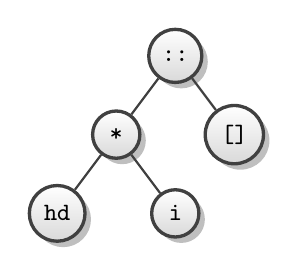
\begin{tikzpicture}
        [font=\small, edge from parent,
        every node/.style={top color=white, bottom color=black!15,
        circle, minimum size=6mm, draw=black!75,
        very thick, drop shadow, align=center},
        edge from parent/.style={draw=black!75,thick},
        level distance=1.0cm]
        \node (cons) {\texttt{::}}
            child { node (mult) {\texttt{*}}
                child { node {\texttt{hd}}}
                child { node {\texttt{i}}}
                }
            child {node (elist) {\texttt{[]}}};
        \end{tikzpicture}
        \subcaption{Fix AST}
        \label{fig:fix_ast}
    \end{minipage}
    \begin{minipage}[c]{0.49\linewidth}
        \centering
        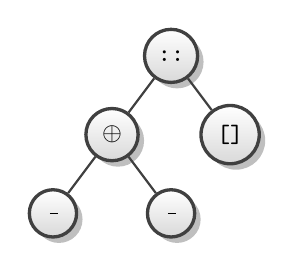
\begin{tikzpicture}
            [font=\small, edge from parent,
            every node/.style={top color=white, bottom color=black!15,
            circle, minimum size=6mm, draw=black!75,
            very thick, drop shadow, align=center},
            edge from parent/.style={draw=black!75,thick},
            level distance=1.0cm]
            \node (cons) {\texttt{::}}
                child { node (mult) {\texttt{$\oplus$}}
                    child { node {\texttt{$\_$}}}
                    child { node {\texttt{$\_$}}}
                    }
                child {node (elist) {\texttt{[]}}};
            \end{tikzpicture}
        \subcaption{Template GAST}
        \label{fig:templ_gast}
    \end{minipage}
    \caption{(left) The fix from example \autoref{fig:mulByDigit} and (right) a possible template for that fix.}
\end{figure}


\subsection{Extracting Fix Templates from a Dataset}
\label{sec:templ-partition:templates}

Our approach fully automates the extraction of fixes by harvesting a set of fix
templates from a training set of program pairs.
%
Given a program pair $(\pbad, \pfix)$ from the dataset, we extract a unique fix
for each location in $\pbad$ that changed in $\pfix$.
%
We do so with an expression-level $\diffsym$~\citep{Lempsink2009-xf} function.
%
Recall that we consider fixes to be replacements of expressions, and
therefore we abstract these extracted changes as our fix templates.

\mypara{Contextual Repairs.}
%
Following Felleisen \emph{et al.}~\cite{Felleisen92}, let $\econtext{}$ be the \emph{context} in which an
expression $e$ appears in a program $p$, \ie the program $p$ with $e$
replaced by a hole $\_$.
%
We write that $p = \context{}{e}$, meaning that if we fill the hole with the
original expression $e$ we obtain the original program $p$.
%
In this fashion, $\diffsym$ finds a \emph{minimal} (in number of nodes)
expression replacement $\efix$ for an expression $\ebad$ in $\pbad$, such that
$\pbad = \context{\pbad}{\ebad}$ and $\context{\pbad}{\efix} = \pfix$.
%
There may be several such expressions, and $\diffsym$ returns all
such changes.

\mypara{Examples.} If $\eapp{f}{x}$ is rewritten to $\eapp{g}{x}$, the context is
$\econtext{} = \eapp{\_}{x}$ and the fix is $g$, since $\context{}{g} = \eapp{g}{x}$.

If $\eapp{f}{x}$ is rewritten to $\eplus{(\eapp{f}{x})}{1}$, the context is
$\econtext{} = \_$, and the fix is the whole expression
$\eplus{(\eapp{f}{x})}{1}$, thus $\context{}{\eplus{(\eapp{f}{x})}{1}} =
\eplus{(\eapp{f}{x})}{1}$. (Even though $\eapp{f}{x}$ appears in
both the original and fixed programs, we consider the application expression
$\eapp{f}{x}$ --- but not $f$ or $x$ --- to be replaced with the $+$ operator.)

\subsection{Partitioning the Templates}

Programs over \lang force similar fixes, such as changes to variable names, to
have identical GASTs. Our next step is to define a notion of program fix
\emph{similarity}. Our definition supports the formation of a small but
widely-applicable set of fix templates. This small set is used to train a repair
predictor.

\label{subsec:partitioning}
% \begin{figure*}
% \begin{minipage}{\textwidth}
% \begin{haskellcode}
% ==data Expr== = Var | Bop Expr Expr | App [Expr] | ...

% ==sim :: Expr -> Expr -> Bool==
% sim Var         Var         = True
% sim (Bop x1 y1) (Bop x2 y2) = sim [x1, y1] [x2, y2] ==||== sim [x1, y1] [y2, x2]
% sim (App xs)    (App ys)    = any (\ys' -> any (\xs' -> sim xs' ys') xss) yss
%     where
%         xss = permutations xs
%         yss = permutations ys
% sim _           _           = False

% ==sim :: [Expr] -> [Expr] -> Bool==
% sim (x:xs) (y:ys) = sim x y && sim xs ys
% \end{haskellcode}
% \end{minipage}
% \caption{$\simil{e_1}{e_2}$ denotes when the GAST $e_1$ is similar to $e_2$.}
% \label{fig:similar}
% \end{figure*}

\mypara{GAST Similarity.}
% %
% \autoref{fig:similar} formalizes a relation that states when
% an expression $e_1$ is \emph{similar to} $e_2$  (written \simil{e_1}{e_2}).
% %
Two GASTs are \emph{similar} when
the root nodes are the same and their child subtrees (if any) can be ordered
such that they are pairwise similar. For example, $x + 3$ and $7 - y$ yield
\emph{similar} GASTs where the root nodes are both abstract binary operators,
one child is an abstract literal, and one child is an abstract variable.
        % \eg $e_{11} \oplus e_{12}$ and $e_{21} \oplus e_{22}$ are
        % similar \textit{iff} $(e_{11}, e_{21})$ and $(e_{12}, e_{22})$ or
        % $(e_{11}, e_{22})$ and $(e_{12}, e_{21})$ are pair-wise similar.

% TODO: partition is novel? compare to previous work
\mypara{Partitioning.}
GAST similarity defines a relation which is reflexive, symmetric, and transitive
and thus an \emph{equivalence} relation. We can now define \emph{partitioning}
as the computation of all possible \emph{equivalence classes} of our extracted
fix templates \wrt GAST similarity. Each class can consist of several
member-expressions and any one of them can be viewed as the class
\emph{representative}. Each representative can then be used as a fix template to
produce repairs for ill-typed programs.

For example, $\hat{x} \oplus \hat{n}$ and $\hat{n} \oplus \hat{x}$ are similar
so they are in the same class. Either one can be used as the representative and
our repair algorithm in \autoref{sec:synthesis} will essentially consider both
when fixing an erroneous program with this template.

Finally, our partitioning algorithm returns the top $N$ equivalence classes
based on their member-expressions frequency in the dataset. $N$ is a parameter
of the algorithm and is chosen to be as small as possible while the top $N$
classes represent a large enough portion of the dataset. We discuss the
appropriate choice of $N$ in \autoref{sec:eval}.

\section{Predicting Fix Templates}
\label{sec:templ-pred}

In this section, we introduce our high-level approach to predicting repair
templates $\T$ for a given location of the program. More formally, our goal is
to define the $\repairsym$ function in \autoref{fig:api}, in terms of the simple
language \repairLang (\autoref{fig:rtl-syntax}), that produces an error location
confidence score and confidence scores for some predefined templates for each
subexpression in a program $e$. The $\repairsym$ function takes some feature
extraction functions $\featuresym$, a dataset $\Dataset$ of program pairs $e
\times e$, a finite list of fix templates $\T$ as inputs and uses internally
three more major functions.

Firstly, the $\extractTsym$ function does the feature extraction from the
program pair dataset and maps each subexpression of the original erroneous
program to a boolean vector. The first entry refers to the error locations that
the user fixed, \ie whether a subexpression changed in a program pair. Those
locations are acquired through the $\diffsym$ function. The rest of the boolean
vector has at most one $\etrue$ value, and corresponds to the fix template $\T$
that used to repair that subexpression.

The $\extractTsym$ function is applied to all the dataset program pairs and all
subexpression feature and label vectors are then grouped together into one
larger \emph{training} dataset. The training dataset is used by the $\trainTsym$
function to produce two predictive models, $\Model$ and $\ModelT$. $\Model$ is
used for error localization and $\ModelT$ for predicting fix templates.

Finally, the $\predictTsym$ function produces an error location confidence score
$\Runit$ and confidence scores $\Tmap{\Runit}$ for each of the selected fix
templates for a specific subexpression in a new program $e$ that we want to
finally repair. The $\predictTsym$ function expects as input the two generated
predictive models and a new feature vector $\V$, that corresponds to a
subexpression's feature vector acquired again by $\extractTsym$. It is then
applied to each subexpression in $e$'s type-error slice (TODO: ref) and
generates a mapping from program expressions to confidence scores $\Emap{(\Runit
\times \Tmap{\Runit})}$ as output of the top-level function $\repairsym$.

% Firstly, a $\ModelT$ is produced by $\trainTsym$, which performs supervised
% learning on a training set of feature vectors $\V$, each assigned a vector of
% (boolean) labels $\B$ that represent the template $\T$ that ``repairs'' the
% location that the feature vector represents. In our case, only one template can
% be used to repair a given location in a program, thus, at most, only one slot of
% the label vector $\B$ can be $\etrue$. This is equivalent to the
% \emph{multi-class classification} problem, where the predictor models have to
% learn to distinguish between several classes. Once trained, we can make
% predictions on new inputs, producing template confidences $\Runit$ for each
% template $\T$.

% Our $\ModelT$s expect feature vectors $\V$ and boolean labels $\B$, both of a
% fixed length for each specific location. Therefore, we define similarly to
% $\extractsym$, the function $\extractTsym$ in \autoref{fig:api}. We use again
% $\diffsym$ to get the set of changed expressions of a given program pair. Those
% are then used by the function $\clustersym$ to get the repair templates by
% grouping different expressions together based on some similarity metric and thus
% reducing their number and making them more concrete. The $\extractTsym$
% function, then, extracts $\featuresym$ from each subexpression, acquired by
% $\diffsym$ but limited to the type-error slice (TODO: ref) and assigns the
% boolean labels based on the templates $\T$ according to $\clustersym$, with only
% one being $\etrue$ at a time

\begin{figure}
\small
\centering
\begin{minipage}[c]{\linewidth}
  \[
  \boxed{
  \begin{array}{rcl}
  e & ::=    & x \spmid \efun{x}{e} \spmid \eapp{e}{e} \spmid \elet{x}{e}{e} \\
    & \spmid & n \spmid \eplus{e}{e}\\
    & \spmid & b \spmid \eif{e}{e}{e} \\
    & \spmid & \epair{e}{e} \spmid \epcase{e}{x}{x}{e} \\
    & \spmid & \enil \spmid \econs{e}{e} \spmid \ecase{e}{e}{x}{x}{e} \\[0.05in]

  n & ::= &  0, 1, -1, \ldots \\[0.05in]

  b & ::= &  \etrue \spmid \efalse \\[0.05in]

  t & ::= & \alpha \spmid \tbool \spmid \tint \spmid \tfun{t}{t} \spmid \tprod{t}{t} \spmid \tlist{t} \\[0.05in]
  \end{array}
  }
  \]
  \captionof{figure}{Syntax of \repairLang}
  \label{fig:syntax}
\end{minipage}
\begin{minipage}[c]{\linewidth}
  \lstDeleteShortInline{|} % sigh...
  \[
  \boxed{
  \begin{array}{lcl}
    \V           & \defeq & \List{\R}\\
    \Runit       & \defeq & \{r \in \R\ |\ 0 \le r \le 1\} \\ % [0,1]\\
    \T           & \defeq & e\\
    \featuresym  & : & \List{e \to \R} \\
    \labelsym    & : & e \times e \to \List{e} \\
    \extractTsym & : & \featuresym \to e \times e \to \List{\V \times \List{\T}} \\
    \trainTsym   & : & \List{\V \times \List{\T}} \to \Model \\
    \predictTsym & : & \Model \to \V \to \List{\Runit} \\
    \midrule
    \repairsym   & : & \Model \to e \to \List{e \times \Runit \times \List{\Runit}}
  \end{array}
  }
  \]
  \lstMakeShortInline{|}
  \captionof{figure}{
    A high-level API for converting program pairs to
    feature vectors and template labels.
  }
  \label{fig:api}
\end{minipage}
\end{figure}


\subsection{Feature and Label Extraction}
\label{subsec:extract}
The first issue we must tackle is formulating our learning task in machine
learning terms. We are given programs over \repairLang, but learning algorithms
expect to work with \emph{feature vectors} $\V$ --- vectors of real numbers,
where each column describes a particular aspect of the input. Thus, our first
task is to convert programs to feature vectors with the $\extractTsym$ function.

Similarly to previous work \citep{Seidel:2017}, we choose to model a program as
a \emph{set} of feature vectors, where each element corresponds an expression in
the program. Thus, given the |mulByDigit| program in \autoref{fig:mulByDigit} we
would first split it into its constituent sub-expressions and then transform
each sub-expression into a single feature vector. We group the features into
five categories, using \autoref{fig:mulByDigit} as a running example of the
feature extraction process.

\mypara{Local syntactic features}
These features describe the syntactic category of each expression $e$. In other
words, for each production of $e$ in \autoref{fig:ml-syntax} we introduce a feature
that is enabled (set to $1$) if the expression was built with that production,
and disabled (set to $0$) otherwise. For example, the \IsNil feature describes
whether an expression is the empty list $\enil$.

We distinguish between matching on a list vs.\ on a pair, as this affects the
typing derivation. We also assume that all pattern matches are well-formed ---
\ie all patterns must match on the same type. Ill-formed match expressions would
lead to a type-error; however, they are already effectively localized to the
match expression itself. We note that this is not a \emph{fundamental}
limitation, and one could easily add features that specify whether a match
\emph{contains} a particular pattern, and thus have a match expression that
enables multiple features.

\mypara{Contextual syntactic features}
These are similar to local syntactic features, but lifted to describe the parent
and children of an expression. For example, the \IsCaseListP feature in
\autoref{fig:mulByDigit} describes whether an expression's \emph{parent} matches on
a list. If a particular $e$ does not have children (\eg a variable $x$) or a
parent (\ie the root expression), we leave the corresponding features disabled.
This gives us a notion of the \emph{context} in which an expression occurs,
similar to the \emph{n-grams} used in linguistic models
\citep{Hindle2012-hf,Gabel2010-el}.

\mypara{Expression size}
We also propose a feature representing the \emph{size} of each expression, \ie
how many sub-expressions does it contain? For example, the \ExprSize feature in
\autoref{fig:mulByDigit} is set to four for the expression |mulByDigit i tl| as it
contains four expressions: the three variables and the application itself. This
allows the model to learn that, \eg, expressions closer to the leaves are more
likely to be blamed than expressions closer to the root.

\mypara{Typing features}
A natural way of summarizing the context in which an expression occurs is with
\emph{types}. Of course, the programs we are given are \emph{untypeable}, but we
can still extract a \emph{partial} typing derivation from the type checker and
use it to provide more information to the model.

A difficulty that arises here is that, due to the parametric type constructors
$\tfun{\cdot}{\cdot}$, $\tprod{\cdot}{\cdot}$, and $\tlist{\cdot}$, there is an
\emph{infinite} set of possible types --- but we must have a \emph{finite} set
of features. Thus, we abstract the type of an expression to the set of type
constructors it \emph{mentions}, and add features for each type constructor that
describe whether a given type mentions the type constructor. For example, the
type $\tint$ would only enable the $\tint$ feature, while the type
$\tfun{\tint}{\tbool}$ would enable the $\tfun{\cdot}{\cdot}$, $\tint$, and
$\tbool$ features.

We add these features for parent and child expressions to summarize the context,
but also for the current expression, as the type of an expression is not always
clear \emph{syntactically}. For example, the expressions |tl| and
|mulByDigit i tl| in \autoref{fig:mulByDigit} both enable \HasTypeList, as they
are both inferred to have a type that mentions $\tlist{\cdot}$.

Note that our use of typing features in an ill-typed program subjects us to
\emph{traversal bias} \citep{McAdam1998-ub}. For example, the |mulByDigit i tl|
expression might alternatively be assigned the type $\tint$. Our models will
have to learn good localizations in spite this bias.

\mypara{Type error slice}
Finally, we wish to distinguish between changes that could fix the error, and
changes that \emph{cannot possibly} fix the error. Thus, we compute a minimal
type-error \emph{slice} for the program (\ie the set of expressions that
contribute to the error) and if the program contains multiple type-errors, we
compute a minimal slice for each error. We then have a post-processing step that
discards all expressions that are not included in those slices.


\mypara{Labels}
Recall that we use two predictive models, $\Model$ for error localization and
$\ModelT$ for predicting fix templates. Thus, we define the output of the
$\Model$ to be a boolean label, where ``false'' means the expression
\emph{should not} change and ``true'' means the expression \emph{should} change.
We also want to assign the correct labels for $\ModelT$. These labels must
represent the repair template $\T$ that was used to fix the input program at a
location $l$. If that location was not changed, all boolean labels are set to
``false''. Therefore, for the purpose of template prediction, we have a
fixed-length boolean vector that represents the fix template used for repairing
a subexpression at a location $l$. This vector has at most one slot set to
``true''.

\subsection{Training Predictive Models}
\label{subsec:train}
\lstDeleteShortInline{|} % sigh...

Our goal with the $\trainTsym$ function is to train two separate
\emph{classifiers} given a training set $S : \List{\V \times \B \times
\Tmap{\B}}$ of labeled examples, one used to predict error locations $\Model$
and the other to predict fix templates $\ModelT$ for an new input program $p$.
Essentially, though, we require that the error localization classifier outputs a
\emph{confidence score} $\Runit$ that represents the probability that the
subexpression in program $p$ it was applied to, is the error that needs to be
fixed. We also require that the fix template classifier outputs a confidence
score $\Runit$ for each of the selected fix templates that measures how sure the
classifier is that a given template can be used to repair the associated
location of the input program $p$.

There are many learning algorithms to choose from, existing on a spectrum that
balances expressiveness with ease of training (and of interpreting the learned
model). In this section we consider a standard learning algorithm: \emph{neural
networks}. A thorough introduction to these techniques can be found in
introductory machine learning textbooks \citep[\eg][]{Hastie2009-bn}.

% Below we briefly introduce each technique by describing the rules it learns, and
% summarize its advantages and disadvantages. For our application, we are
% particularly interested in three properties -- expressiveness, interpretability
% and ease of generalization. Expressiveness measures how complex prediction rules
% are allowed to be, and interpretability measures how easy it is to explain the
% cause of prediction to a human. Finally ease of generalization measures how
% easily the rule generalizes to examples that are not in the training set; a rule
% that is not easily generalizable might perform poorly on an unseen test set even
% when its training performance is high.


\mypara{Neural Networks}
The model that we use is a type of neural network called a \emph{multi-layer
perceptron} (see \citep{Nielsen2015-pu} for an introduction to neural networks).
A multi-layer perceptron can be represented as a directed acyclic graph whose
nodes are arranged in layers that are fully connected by weighted edges. The
first layer corresponds to the input features, and the final to the output. The
output of an internal node $v$ is
\[ h_v = g\,(\sum_{j \in N(v)}\!W_{jv} h_j ) \] where $N(v)$ is the set of nodes
in the previous layer that are adjacent to $v$, $W_{jv}$ is the weight of the
$(j, v)$ edge and $h_j$ is the output of node $j$ in the previous layer. Finally
$g$ is a non-linear function, called the activation function, which in recent
work is commonly chosen to be the \emph{rectified linear unit} (ReLU), defined
as $g(x) = \mathsf{max}(0,x)$ \citep{Nair2010-xg}. The number of layers, the
number of neurons per layer, and the connections between layers constitute the
\emph{architecture} of a neural network. In this work, we use relatively
\emph{deep neural networks} (\dnn) which have an input layer, three hidden layers and
an output layer.

% A major advantage of neural networks is their ability to discover interesting
% combinations of features through non-linearity, which significantly reduces the
% need for manual feature engineering, and allows high expressivity. On the other
% hand, this makes the networks particularly difficult to interpret and also
% difficult to generalize unless vast amounts of training data are available.

\mypara{Multi-class \dnn{}s}
While the above model is enough for error localization (since we have to select
from a binary option), some adjustments on the output layer must be applied. We
again use a deep neural networks for our template prediction $\ModelT$s, but the
output here is a $N$-length vector and therefore the output layer has $N$ nodes.
For multi-class classification problems solved with neural network techniques,
usually a \emph{softmax} function is used for the output layer
\citep{Goodfellow-et-al-2016, Bishop-book-2006}. Softmax assigns decimal
probabilities to each class that must add up to 1.0. This additional constraint
helps training converge more quickly than it otherwise would.

For an output vector $y = (y_1, \dots, y_N) \in \R^{N}$, the standard softmax
function is defined as:
\[ \sigma(y)_i = \frac{e^{y_i}}{\sum_{j=1}^{N} e^{y_j}},\ for\ i = 1, \dots, N \]

The number of neurons per layer are left as the model's hyper-parameters, but we
choose again a deep architecture with three layers, and with each layer having
more neurons than the respective error-localization models, with the exact
number needing some tuning.

% TODO: it feels like something is missing (beside the examples)


\subsection{Predicting Fix Templates}
\label{subsec:predict}

Our ultimate goal is to be able to pinpoint what parts of an erroneous program
should be repaired and what fix templates should be utilized for that purpose.
Therefore, the $\repairsym$ function uses $\predictTsym$ to predict all
subexpressions' confidence scores $\Runit$ to be an error location and
confidence scores $\Tmap{\Runit}$ for each of the selected fix templates. In
this section we show how all the functions in our high-level API in
\autoref{fig:api} are combined to produce a final list of confidence scores for
a new program $P$.

\mypara{The Prediction Algorithm}
Our algorithm firstly extracts the machine learning appropriate dataset $D_{ML}$
from the program pairs dataset $D$. For each program pair in $D$, the
$\extractTsym$ function returns a mapping from the erroneous program's
expression to a feature and label vector. The function
$\textsc{GetSubEsInTESlice}$ only keeps the expressions in the the type-error
slice and returns a list of the respective feature and label vectors, which is
then added in the $D_{ML}$ dataset. The $D_{ML}$ dataset is used by the
$\trainTsym$ function to generate our predictive $Models$. At this point we have
to perform again the feature extraction for a new program $P$, not included
before in our dataset $D$. Thus we use again $\extractTsym$, by providing
program $P$ twice, since in the case we don't have a program as we are trying to
produce the final repair. After acquiring again only the expression that we find
in the type-error slice and therefore ignoring the label vectors, we apply the
$\predictTsym$ function in each feature vector $v$, that corresponds to an
expression in the type-error slice of $P$. The predicted confidence scores are
then accumulated into the $EMap$ mapping, which is used by our synthesis
algorithm in \autoref{sec:synthesis} to correlate expressions in $P$ with their
confidence scores.

\begin{algorithm}[t]
    \caption{Predicting Templates Algorithm}
    \label{algo:predict-algo}
    \renewcommand{\algorithmicrequire}{\textbf{Input:}}
    \renewcommand{\algorithmicensure}{\textbf{Output:}}
    \begin{algorithmic}[1]
    \Require{Feature Extraction Functions $F$, Fix Templates $Ts$, Program Pair Dataset $D$}
    \Ensure{Predictor $Pr$}
    \Procedure{Predict}{$F,\,Ts,\,D$}
    \State $D_{ML} \gets \emptyset$
    \ForAll{$\pbad \times \pfix \in D$}
      \State $d \gets$ \Call{Extract}{$F,\,Ts,\,\pbad \times \pfix$}
      \State $D_{ML} \gets D_{ML}\,\cup$ \Call{InSlice}{$\pbad,\,d$}
    \EndFor
    \State $Models \gets$ \Call{Train}{$D_{ML}$}
    \State $Data \gets \lambda p.$ \Call{InSlice}{$p,$ \Call{Extract}{$F,\,Ts,\,p \times p$}}
    \State $Pr \gets \lambda p.$ \Call{Map}{$\lambda \tilde{p}.$ \Call{Rank}{$Models,\,\tilde{p}[0]$}, $Data(p)$}
    \State \Return{$Pr$}
    \EndProcedure
    \end{algorithmic}
\end{algorithm}


\section{Repair Synthesis from Templates}
\label{sec:synthesis}
We use an \emph{enumerative} program synthesis algorithm to fully repair a
program using the predicted templates and locations of our neural network
models. In \autoref{subsec:location-rank}, we show how we fix \emph{multiple}
error locations in a single program, and in \autoref{subsec:local-synthesis}, we
present our synthesis algorithm for producing \emph{local repairs} for a given
program location.
% Finally, we briefly show in \autoref{subsec:repair} how we use the
% aforementioned techniques to \emph{fully repair} an ill-typed program.

\subsection{Ranking Error Locations}
\label{subsec:location-rank}

\mypara{Error Location Confidence}
Recall from \autoref{sec:templ-pred} that for each location in a program's
type-error slice, our $\Model$ generates a confidence score $\Conf$ of that
location containing an error that needs to be fixed, and our $\ModelT$ generates
the repair templates' confidence scores.

% Our synthesis algorithm attempts to repair the program location with the
% highest confidence score $\Conf$. To do so, it produces repairs
% using each of the first $N$ templates in descending order of confidence
% (in our implementation, $N=6$). If none of these templates
% allow it to synthesize a program that type-checks, it considers the next
% program location (in decreasing order of confidence), until it succeeds.
Our synthesis algorithm ranks all program locations based on their confidence
scores $\Conf$. For all locations in descending order of their confidence
scores, a fix template is used to produce a repair. Fix templates are also
considered in descending order of confidence. If the algorithm fails to
synthesize a program that type-checks, the next location is considered, until it
succeeds.

\mypara{Multiple Error Locations}
In practice, frequently more than one location needs to be repaired. We thus
extend the above approach to fix programs with multiple error locations.

Let the confidence scores $\Conf$ for all locations in the type error slice from
our error localization model $\Model$ be $(l_1, c_1), \dots, (l_k, c_k)$, where
$l_i$ is a program location and $c_i$ its confidence score. We assume for
simplicity that the probabilities $c_i$ are independent, so
the probability that \emph{all} the locations $\{l_i \dots l_j\}$ need to be fixed
is the product $c_i \cdots c_j$. Therefore, instead of
just ranking and trying to find fixes for single locations $l$,
we use \emph{sets} of locations ($\{l_i\}, \{l_i, l_j\}, \{l_i, l_j, l_k\}$, \etc),
ranked by the products of their confidence scores.
% In practice we only consider up to \emph{five} locations to be fixed
% simultaneously; any more than that takes too much time to generate and has too
% small a chance of leading to a good solution.


\subsection{Local Synthesis from Templates}
\label{subsec:local-synthesis}

\mypara{Enumerative Program Synthesis}
Our synthesis algorithm is a classic \emph{enumerative} program synthesis method
guided by an input template. Enumerative synthesis searches all possible
expressions over a language until a high-level
specification is reached. In our case, we only try to synthesize a part of the
program that already captures the intent of the user and therefore our only
specification is that the repaired program is type-safe. However, we can also
extend this specification by allowing our algorithm to search for programs that
have the user's desired type signature.

Given a location $l$ and a template $t$, our algorithm searches over all
possible expressions over \lang that will satisfy those goals by generating a
\emph{local repair} that expands $t$'s GAST. One advantage of this technique
is that we can exploit the expression $e$ at location $l$ to further guide our
synthesis, since subexpressions used by the programmer at $l$ are usually reused
for their final repair.

\begin{algorithm}[t]
    \caption{Local Repair Algorithm}
    \label{algo:local-repair-algo}
    \renewcommand{\algorithmicrequire}{\textbf{Input:}}
    \renewcommand{\algorithmicensure}{\textbf{Output:}}
    \begin{algorithmic}[1]
    \Require{Language Grammar \lang, Program $P$, Template $T$, Repair Location $L$, Max Repair Depth $D$}
    \Ensure{Local Repairs $R$}
    \Procedure{Enumerate}{$\lang, P, T, L, D$}
    \State $R \gets \emptyset$
    \ForAll{$d \in [1 \dots D]$}
      \State $\tilde{\alpha} \gets$ \Call{NonTerminalsAt}{$T, d$}
      \ForAll{$\alpha \in$ \Call{RankNonTerminals}{$\tilde{\alpha}, P, L$}}
        \If{\Call{IsHole}{$\tilde{\alpha}$}}
          \State $Q \gets$ \Call{GrammarRules}{$\lang$}
          \State $\tilde{\beta} \gets \{\beta\:|\:(\alpha, \beta) \in Q\}$
          \ForAll{$\beta \in$ \Call{RankRules}{$\tilde{\beta}, T$}}
            \State $\hat{T} \gets$ \Call{ApplyRule}{$T, (\alpha, \beta)$}
          \EndFor
        \Else
          \ForAll{$\sigma \in$ \Call{GetTerminals}{$P, \alpha, \lang$}}
            \State $\hat{T} \gets$ \Call{ReplaceNode}{$T, \alpha, \sigma$}
          \EndFor
        \EndIf
        \State $\hat{P} \gets$ \Call{ReplaceExprAt}{$P, L, \hat{T}$}
        \If{\Call{TypeCheck}{$\hat{P}$}}
          \State $R \gets R \cup \{\hat{P}\}$
        \EndIf
      \EndFor
    \EndFor
    \State \Return{$R$}
    \EndProcedure
    \end{algorithmic}
\end{algorithm}


\mypara{Generating Local Repairs with Templates}
Using our \textsc{Enumerate} method (\autoref{algo:local-repair-algo}), we lazily generate local repairs $R$ for
each subset of locations that is highest in confidence score. The
\textsc{Enumerate} method starts to fill in a template $T$ for location $L$ of
the program $P$ based on the context-free grammar $\lang$. It starts from the
parent node at the first level of the template $T$ and incrementally moves
down the tree. When a hole is found in the tree, the algorithm tries to expand
the tree one more level using $\lang$'s production rules $Q$. The production
rules are considered in an ranked order based on the subexpressions that already
appear in $P$'s location $L$ and the template $T$. It then applies the rule to the
template $T$. If the node $\tilde{\alpha}$ was not a hole, terminals from the
program $P$, the expression $\alpha$ at the location $L$ and the grammar
$\lang$ are used to fill that node, depending on what terminals were used from
$\repairLang$. For example, $\repairLang$'s operator $\oplus$ can be replaced
with $+,\:-,\:\etc$

After the template $T$ had some changes applied to it \BC{too vague}, we get an
\emph{instantiated} template $\hat{T}$, which then replaces the expression at
location $L$. If the new program $\tilde{P}$ type-checks, it is inserted into
the list of generated solutions $R$. $R$ is
generated lazily in practice and the top-N can be requested for the user
depending on the level of feedback that is needed.


% \subsection{Program Repair}
% \label{subsec:repair}

% \mypara{Combining Error Localization and Local Repairs}

\section{Evaluation}
\label{sec:eval}

\lstMakeShortInline[mathescape=true]{|}

We have implemented analytic program repair in \toolname: a system for
repairing type errors for a purely functional subset of \ocaml. Next,
we describe our implementation and an evaluation that addresses three
questions:

\begin{itemize}
    \item \textbf{RQ1}: How \emph{accurate} are \toolname's predicted repairs?
                        (\S~\ref{sec:eval:accuracy})
    \item \textbf{RQ2}: How \emph{efficiently} can \toolname synthesize fixes?
                        (\S~\ref{sec:eval:efficiency})
    \item \textbf{RQ3}: How \emph{useful} are \toolname's error messages?
                        (\S~\ref{sec:eval:useful})
    \item \textbf{RQ4}: How \emph{precise} are \toolname's template fixes?
                        (\S~\ref{sec:eval:template_quality})

\end{itemize}

% \subsection{Implementation} \label{sec:eval:gen_method}

\mypara{Training Dataset}
%
For our evaluation, we use an \ocaml dataset gathered from an undergraduate
Programming Languages university course, previously used in related work
\citep{Seidel2017-ko,Seidel:2017}. It consists of erroneous programs and their
subsequent fixes and is divided in two parts; the Spring 2014 class (\SPRING)
and the Fall 2015 class (\FALL). The homework required students to write 23
distinct programs that demonstrate a range of functional programming idioms, \eg
higher-order functions and (polymorphic) algebraic data types.

\mypara{Feature Extraction}
%
\toolname represents programs with BOAT vectors over a set of 449
% WRW notes: the text had 416, but if you sum all of the subparts you get 449
features from
each sub-expression in a program: 45 local syntactic, 315
contextual, 88 typing features, and 1 expression size feature.
For contextual features, for each subexpression we
additionally extract the local syntactic features of its first 4
(left-to-right) children. In addition, we extract those features for its
ancestors, starting from its parent and going up to two more parent nodes.
    % If an expression does not have a ancestor or children, these features will
    % simply be disabled. If an expression has more than four children, the
    % classifiers will receive no information about the additional children.
    %
For typing features, we support |int|s, |float|s, |char|s, |string|s, and
    the user-defined |expr|. These features are extracted for each
    sub-expression and its context.
%
% 1 feature denoting the size of each subexpression.

\mypara{Dataset Cleaning}
%
We extract fixes as expressions replacements over a program pair using \diffsym.
A disadvantage of using \diffsym s with this dataset is that some students may
have made many, potentially unrelated, changes between compilations; at some
point the ``fix'' becomes a ``rewrite''. These rewrites can lead to meaningless
fix templates and error locations. We discard such outliers when the fraction of
subexpressions that have changed in a program is more than one standard
deviation above the mean, establishing a diff threshold of 40\%. We also discard
programs that have changes in 5 or more locations, noting that even
state-of-the-art multi-location repair techniques cannot reproduce such
``fixes'' \citep{Saha_2019}. The discarded changes account for roughly 32\% of each
dataset, leaving 2,475 program pairs for \SPRING and 2,177 pairs for \FALL.
Throughout, we use \SPRING as a training set and \FALL as a test set.

\mypara{\dnn based Classifier}
%
\toolname's template prediction uses a multi-layer neural network \dnn based
classifier with three fully-connected hidden layers of 512 neurons. The neurons
use rectified linear units (ReLU) as their activation function
\citep{Nair2010-xg}.
%
The \dnn was trained using \emph{early stopping} \citep{Hastie2009-bn}: training
is stopped when the accuracy on a distinct small part of the training set is not
improved after a certain amount of epochs (5 epochs, in our implementation).
%
We set the maximum number of epochs to 200.
%
We used the \textsc{Adam} optimizer \citep{Kingma2014-ng},
a variant of stochastic gradient descent that converges faster.

\subsection{RQ1: Accuracy}

\label{sec:eval:accuracy}

Most developers will consider around five or six suggestions before falling back
to manual debugging \citep{Kochhar2016-oc,Parnin2011-ce}.
%
Therefore, we consider \toolname's accuracy up to the \emph{top six} fix
template prediction, \ie predicted fix templates that represent the user's
actual fix.

\mypara{Baselines}
%
We compare \toolname's \dnn-based predictor against two baseline classifiers: a
\random classifier that returns templates chosen uniformly at random from the 50
templates learned from the \SPRING training dataset, and a \popular classifier
that returns the most popular templates in the training set in decreasing order.

\mypara{Results: Accuracy of Prediction}
%
\autoref{fig:accuracy-results} shows the accuracy results of our template
prediction experiments. The y-axis describes the fraction of \emph{erroneous}
sub-terms (locations) for which the actual repair was one of the top-K predicted
repairs.
%
The naive baseline of selecting templates at random achieves
\RandomTopOne\% Top-1 accuracy (\RandomTopSix\% Top-6), while
the \popular classifier achieves a Top-1 accuracy of \PopularTopOne\%
(\PopularTopSix\% Top-6).
%
Our \dnn classifier significantly outperforms these naive classifiers, ranging
from \DnnTopOne\% Top-1 accuracy to \DnnTopSix\% Top-6 accuracy.
%
In fact, even with only \dnn's first prediction one outperforms top 6
predictions of both \random and \popular.
%
The \random classifier's low performance is as expected.
%
The \popular classifier performs better: some homework assignments were shared
between \SPRING and \FALL quarters and, while different groups of students
solved these problems for each quarter, the novice mistakes that they made seem
to have a pattern. Thus, the most \emph{popular ``fixes''} (and therefore the
relevant templates) from \SPRING were also popular in \FALL.

% colors from http://colorbrewer2.org/?type=sequential&scheme=Blues&n=3
\definecolor{blue1}{HTML}{DEEBF7}
\definecolor{blue2}{HTML}{9ECAE1}
\definecolor{blue3}{HTML}{3182BD}
\definecolor{green1}{HTML}{E5F5E0}
\definecolor{green2}{HTML}{A1D99B}
\definecolor{green3}{HTML}{31A354}

\begin{figure}[t]
\centering
\begin{tikzpicture}
\begin{axis}[
  ybar stacked,
  % width=\linewidth,
  height=6cm,
  % title={Accuracy of Repair Template Prediction},
  ylabel={Accuracy},
  bar width=0.82cm,
  ymin=0.0,
  ymax=100.0,
  ytick={0.0, 10.0, 20.0, 30.0, 40.0, 50.0, 60.0, 70.0, 80.0, 90.0, 100.0},
  yticklabel={\pgfmathparse{\tick}\pgfmathprintnumber{\pgfmathresult}\,\%},
  ytick style={draw=none},
  ymajorgrids = true,
  symbolic x coords={random, popular, dnn},
  enlarge x limits=0.5,
  xtick=data,
  xtick style={draw=none},
  xticklabels={\random, \popular, \dnn},
  %x tick label style={rotate=45, anchor=north east},
  x tick label style={font=\small},
  y tick label style={font=\small},
  reverse legend,
  transpose legend,
  legend style={legend pos = north west, legend columns=4, font=\small},
]

\addplot[draw=black, fill=blue1] coordinates {(random, 2.35646958011996552) (popular, 14.438731790916881) (dnn, 44.64438731790917)};
\addlegendentry{Top-1}
\addplot[draw=black, fill=blue2] coordinates {(random, 3.6846615252784924) (popular, 14.395886889460153) (dnn, 24.250214224507282)};
\addlegendentry{Top-3}
\addplot[draw=black, fill=blue3] coordinates {(random, 6.212510711225363) (popular, 11.825192802056556) (dnn, 11.482433590402735)};
\addlegendentry{Top-6}

\end{axis}
\end{tikzpicture}
\caption{
  Results of our template prediction classifiers using the \emph{50 most
  popular} templates. We present the results up to the top 6 predictions, since
  our synthesis algorithm considers that many templates before falling to a
  different location.
}
\label{fig:accuracy-results}
\end{figure}


\begin{figure}[t]
  \centering
  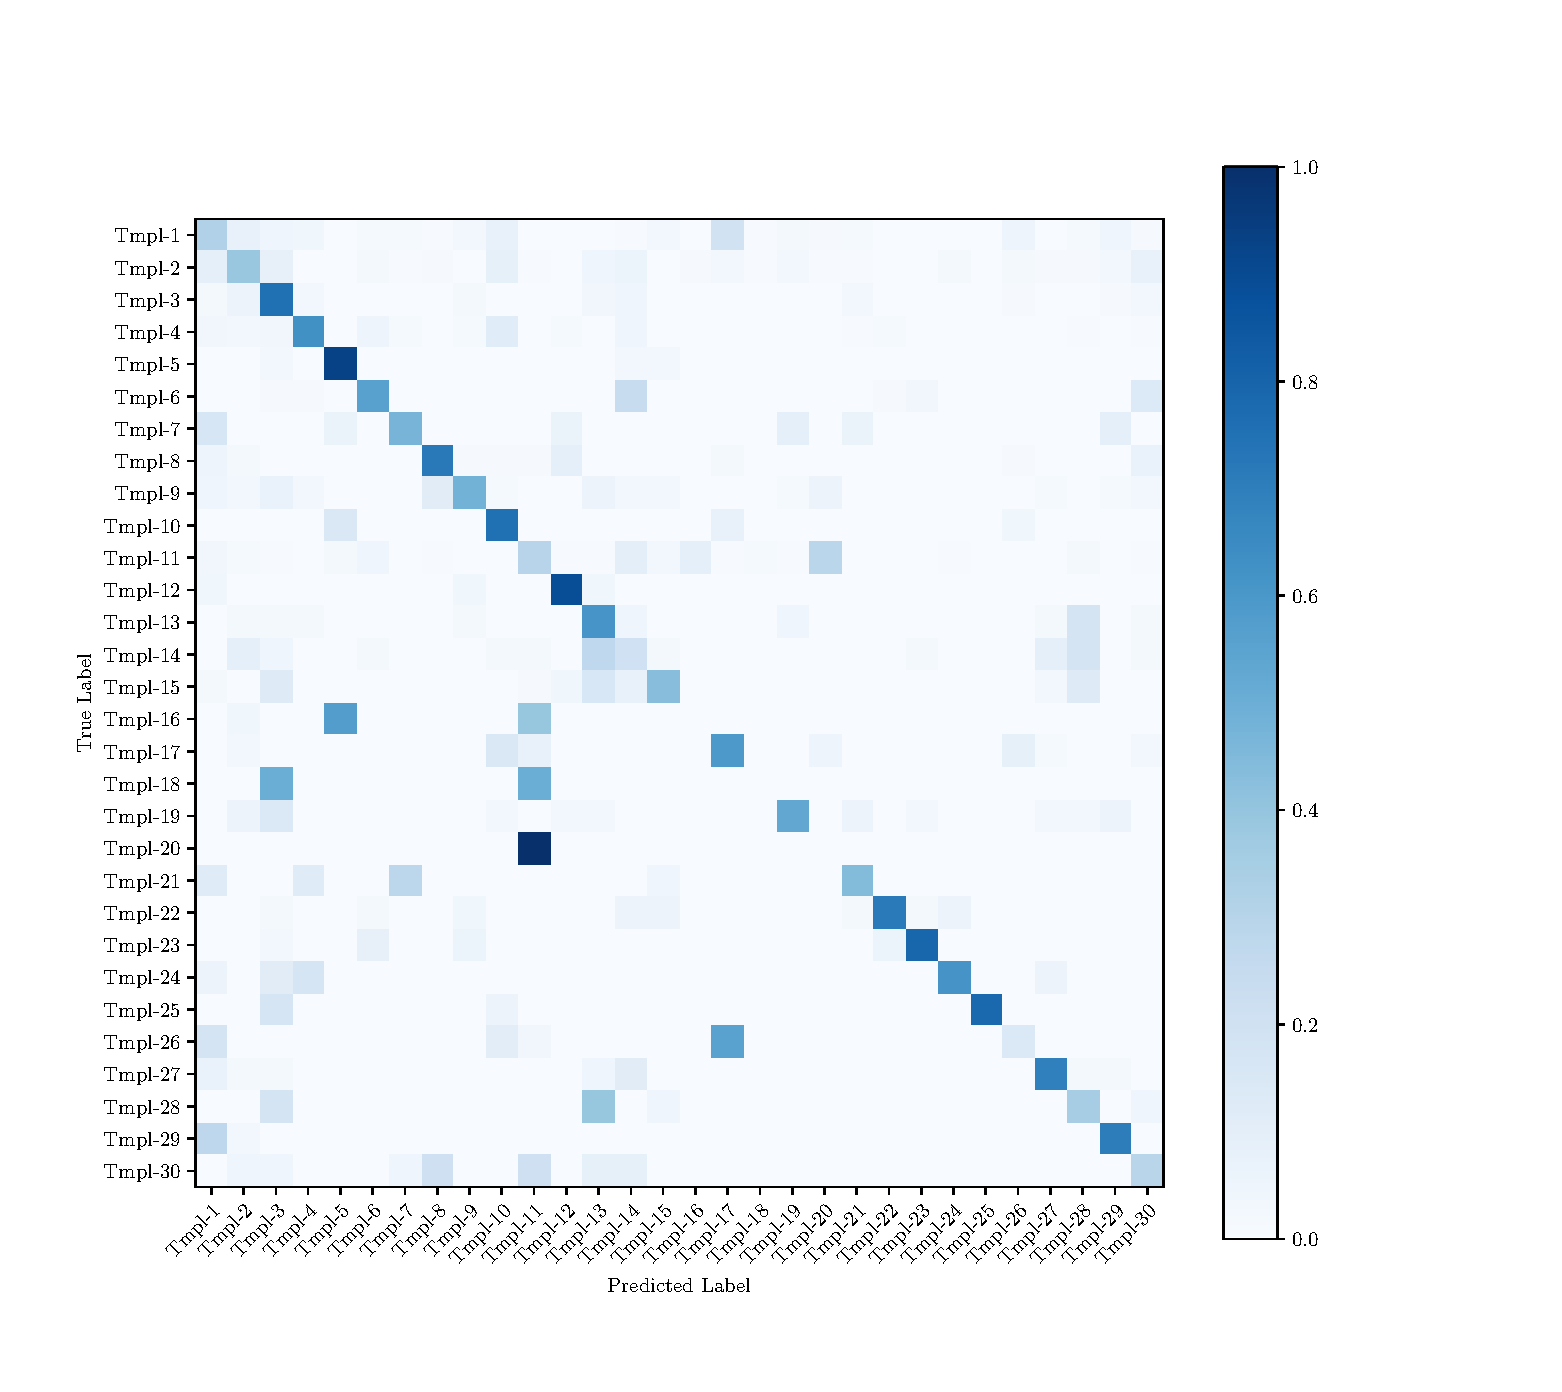
\includegraphics[trim={30 40 100 70},clip,height=2.2in]{evaluation-conf-matrix-no-title.pdf}
  \caption{The confusion matrix of the \emph{top 30} templates. Bolder parts of
  the heatmap show templates that are often mis-predicted with another template.
  The bolder the diagonal is, the more accurate predictions we make.}
  \label{fig:conf-matrix}
\end{figure}

\mypara{Results: Template ``Confusion''}
%
The \emph{confusion matrix} of the each location's top prediction shows which
templates our models mix up.
%
\autoref{fig:conf-matrix} shows this matrix for the top 30 templates acquired
from the \SPRING training set and were tested on the \FALL dataset.
%
Note that most templates are predicted correctly and only a few of them are
often mis-predicted for another template.
%
For example, we see that programs that require template 20
(\elet{\hat{z}}{\epcases{\hat{t}}{\hat{x}}{\hat{y}}{\hat{a}}}{\_}) to be fixed,
almost always are mis-predicted with template 11 (\elet{(\hat{x},
\hat{y})}{\hat{t}}{(\_,\ \_)}). We observe that these templates are still very
similar, with both of them having a top-level |let| that manipulates tuples
$\hat{t}$.

\begin{framed}
  \noindent \toolname's learns correlations between program features and repair
  templates, yielding almost \emph{2x higher} accuracy than the baseline; by
  abstracting programs into features, \toolname is able to \emph{generalize}
  across years and different kinds of programs.
\end{framed}


\subsection{RQ2: Efficiency}
\label{sec:eval:efficiency}
\label{subsec:eval:man_rep_qual_eval}

Next we evaluate the efficiency of \toolname by measuring how many programs it
is able to generate a (well-typed) repair for.
%
To measure efficiency, we limit the synthesizer to 90 seconds for repair
computations.
(In general the procedure is undecidable, and we
conjecture that a longer timeout will diminish the practical usability for
novices.)
%
Recall that the repair synthesis algorithm is guided by the repair template
predictions.
%
We evaluate the efficiency of \toolname by comparing
it against a baseline \naive implementation that, given the predicted fix
location, attempts to synthesize a repair from the trivial ``hole'' template
$\_$.

\autoref{fig:rite_naive} shows the cumulative distribution function of
\toolname's and \naive's repair rates over their synthesis time. We observe that
using the predicted templates for synthesis allows \toolname to generate
type-correct repairs for almost 60\% of the programs in under 10 seconds, which
is nearly 10 points higher than the \naive baseline. We also observe that
\toolname successfully repairs around 10\% more programs than \naive
for execution times greater than 10 seconds.

\begin{framed}
  \noindent \toolname can generate type-correct repairs for the majority of
  ill-typed programs in under 10 seconds.
\end{framed}

% The 11.85\% of the programs that fail to be repaired within that amount of time
% fall in the case of the combined failure of our predictive models to give high
% confidence scores to the correct locations and templates, thus making synthesis
% very expensive.

% \begin{table}
%   \centering
%   \begin{tabular}{l|ccc}
%     Classifier & Completed & Repair Rate & Time (sec) \\
%     \hline
%     \naive   & 77.86\% & 74.78\% & 11.72 \\
%     \toolname & 88.15\% & 84.80\% & 8.81 \\
%   \end{tabular}
%   \caption{Experimental results of \toolname's synthesis.}
%   \label{tab:rite_naive}
% \end{table}

\begin{figure}
  \centering
  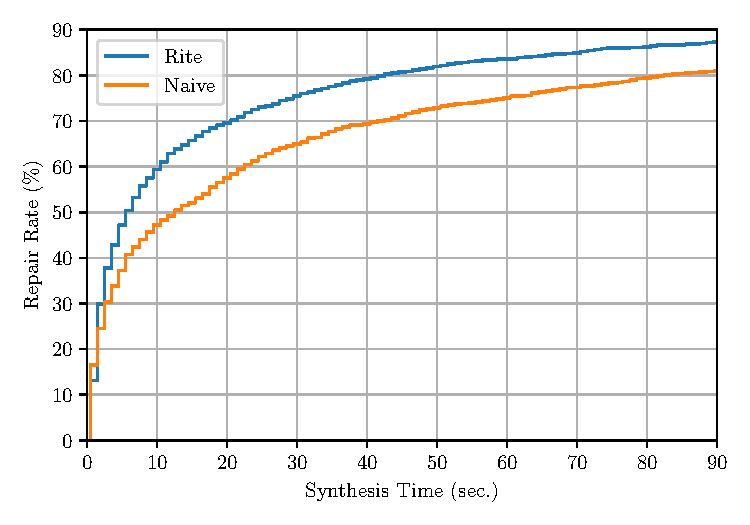
\includegraphics[height=2.2in]{cdf.pdf}
  \caption{The proportion of the test set that can be repaired within a given time.}
  \label{fig:rite_naive}
\end{figure}

\subsection{RQ3: Usefulness}
\label{sec:eval:useful}

The primary outcome is whether the repair-based
error messages generated by \toolname were actually useful to novices.
%
To assess the quality of \toolname's repairs, we conducted an online human
study with 29 participants.
%
Each participant was asked to evaluate the quality of the program fixes
and their locations against a state-of-the-art baseline
(\seminal ~\citep{Lerner2007-dt}).
%
For each program, beyond the two repairs, participants were presented
with the original ill-typed program, along with the standard \ocaml
compiler's error message and a short description of what the original
author of the program intended it to do.
%
From this study, we found that both the edit locations and final
repairs produced by \toolname were better than
\seminal's in a statistically significant manner.

\mypara{User Study Setup}
%
Study participants were recruited from two public research
institutes (names elided for blind review), and was advertised on Twitter.
%
Participants had to assess the quality of, and give comprehensible
bug descriptions for, at least 5 / 10 stimuli. The study took around
25 minutes to complete. Participants were compensated by entering a
drawing for an Amazon Echo voice assistant. There were 29 valid participants.
%
We created the stimuli by randomly selecting a corpus of 21 buggy programs
from the 1834 programs in our dataset where repairs were synthesized.
%
From this corpus, each participant was shown 10 randomly-selected buggy
programs, and two candidate repairs: one generated by \toolname and one
by \seminal.
%
For both algorithms, we used the highest-ranked solution returned.
%
Participant were always unaware which tool generated which candidate
patch.
%
Participants were then asked to assess the quality of each
candidate repair on a Likert scale of 1 to 5 and were asked
for a binary assessment of the quality of each repair's edit
location.
%
We also collected self-reported estimates of both programming and
\ocaml-specific experience as well as qualitative data assessing factors
influencing each participant's subjective judgment of repair quality.
%
From the 29 participants, we collected 554 patch quality assessments,
277 each for \toolname and \seminal generated repairs.

%\begin{figure}
%  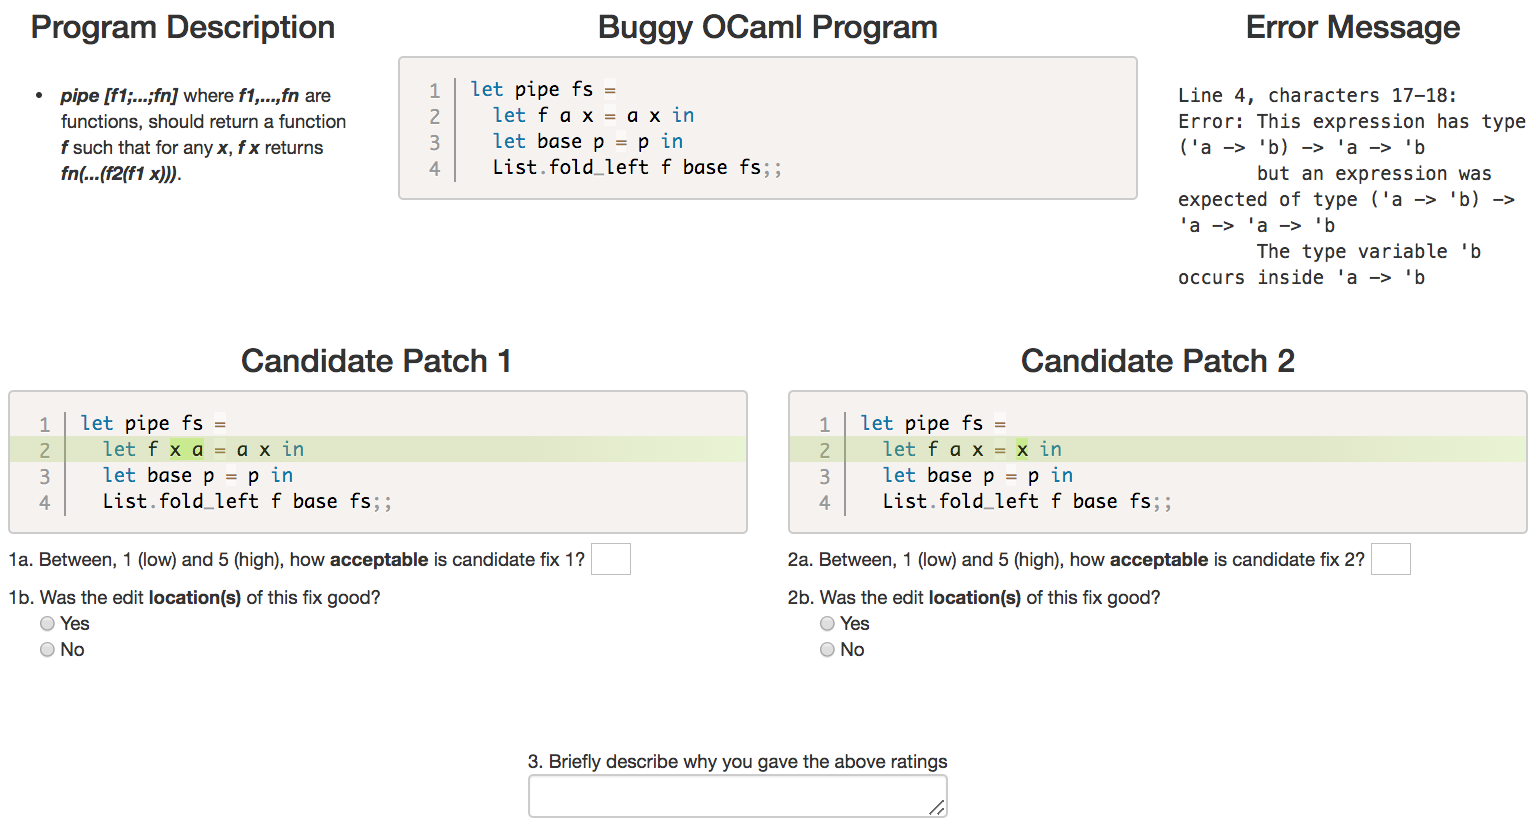
\includegraphics[width=8cm]{SampleStimuli.png}
%  \caption{A sample stimulus used for assessing repair quality.}
%  \label{fig:stimulus}
%\end{figure}

\mypara{Results}
%
In a statistically-significant manner, humans perceive that
\toolname's fault localization and final repairs are both
of higher quality than those produced by \seminal ($p=0.030$
and $p=0.024$ respectively).~\footnote{All tests for statistical
significance used the Wilcoxon signed-rank test.}
%
Regarding fault localization, we find that humans agreed
with \toolname-identified edit locations 81.6\% of the time
but only agreed with those of \seminal 74.0\% of the time.
%
% This 10\% increase is important because \ME{You should explain why this matters.}
%
As for the final repair, humans also preferred \toolname's patches
to those produced by \seminal. Specifically, \toolname's repairs
achieved an average quality rating of 2.41/5 while \seminal's
repairs had an average rating of only 2.11/5, a 14\% increase ($p=0.030$),
showing a statistically-significant improvement over \seminal.

\begin{figure*}
\begin{subfigure}[t]{.33\textwidth}
\centering
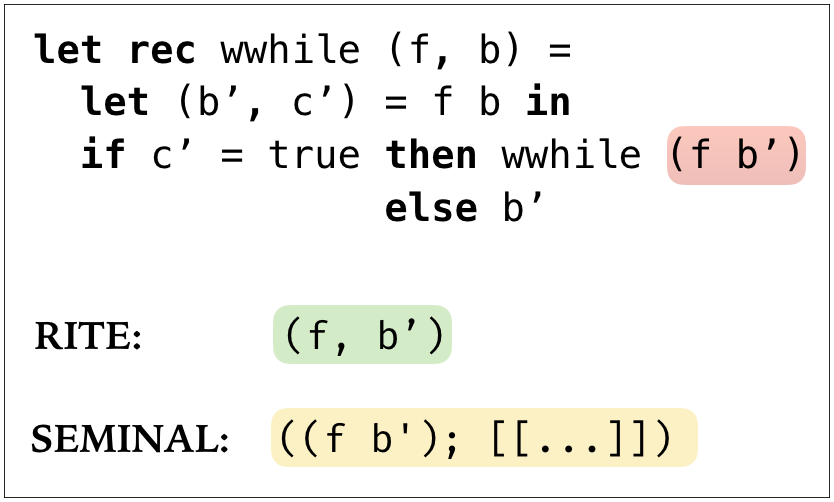
\includegraphics[height=1.4in]{comp1.png}
\caption{\toolname (4.5/5) better than \seminal(1.1/5) with 12 responses $p=0.002$.}
\label{subfig:good1}
\end{subfigure}
\begin{subfigure}[t]{.33\textwidth}
\centering
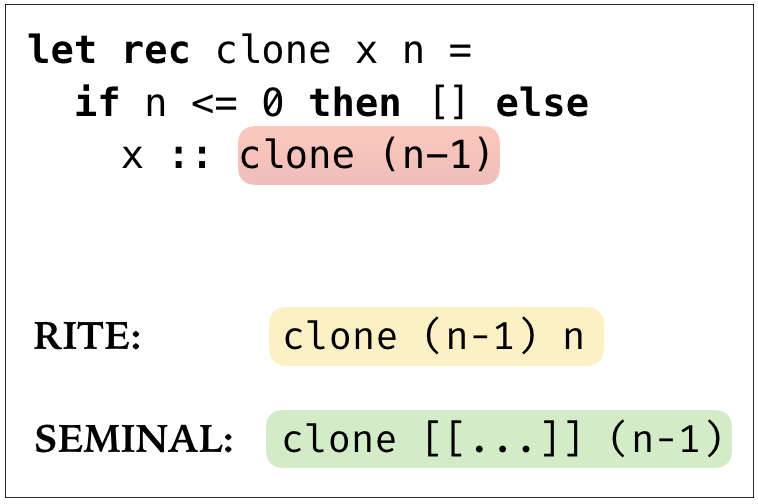
\includegraphics[height=1.4in]{comp2.png}
\caption{\toolname (1.5/5) worse than \seminal(4.1/5) with 18 responses $p=0.0002$.}
\label{subfig:bad}
\end{subfigure}
\begin{subfigure}[t]{.29\textwidth}
\centering
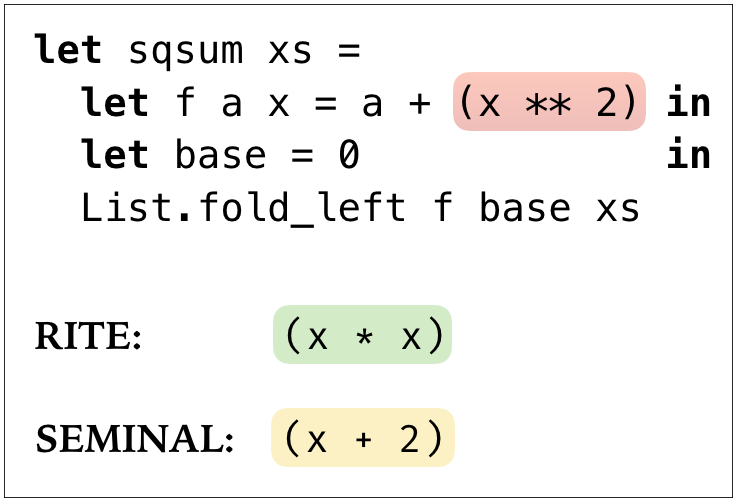
\includegraphics[height=1.4in]{comp3.png}
\caption{\toolname (4.8/5) better than \seminal(1.2/5) with 17 responses $p=0.0003$.}
\label{subfig:good2}
\end{subfigure}
\end{figure*}

\mypara{Qualitative Comparison}
%
We consider several case studies where there were
statistically-significant differences between
the human ratings for \toolname's and \seminal's
repairs.
%
The task in Figure~\ref{subfig:good1} is that
\texttt{wwhile(f, b)} should return $x$ where
there exist values $v_0,...,v_n$ such that:
$b = v_0$, $x = v_n$, and for each $i$ between
0 and $n-2$, we have $f v_i = (v_i+1, true)$
and $f v_n-1 = (v_n, false)$.
%
The task in Figure~\ref{subfig:bad} is to
return a list of \texttt{n} copies of \texttt{x}.
%
The task in Figure~\ref{subfig:good2} is to
return the sum of the squares of the numbers
in the list \texttt{xs}.
%
Humans rated \toolname's repairs better
for the programs in Fig~\ref{subfig:good1}
and~\ref{subfig:good2}.
%
In both cases, \toolname's found a solution
which typechecks and conforms to the problem's
semantic specification.
%
\seminal, however, found a repair that was
either incomplete (\ref{subfig:good1}) or
semantically incorrect (\ref{subfig:good2}).
% FIXME: Add what good thing about \toolname caused this.
On the other hand, in ~\ref{subfig:bad}, \toolname
does worse as the \emph{second} parameter should
be \verb|n-1|. In fact, \toolname's second ranked
repair is the correct one, but it is equal
to the first in terms of edit distance.

\begin{framed}
\noindent Humans perceive both \toolname's edit locations
 and final repair quality to be better than those produced
 by \seminal, a state-of-the-art \ocaml repair tool, in a
 statistically-significant manner.
\end{framed}

\subsection{RQ4: Impact of Templates on Quality}
\label{sec:eval:template_quality}

Finally, we seek to evaluate whether \toolname's template-guided
approach is really at the heart of its effectiveness. To do so,
as in \S~\ref{sec:eval:efficiency}, we performed an assessment
to compare the results of using \toolname's error messages
synthesized from predicted templates to those generated by
a \naive synthesizer that returns the first well-typed term
(\ie synthesized from the trivial $\_$ template).

\mypara{User Study Setup}
%
For this user study, we used the same corpus of 21 buggy programs
randomly chosen in \S~\ref{sec:eval:useful}. For each of the
programs we generated three messages: using \toolname, using \seminal,
and using the \naive approach but at the \emph{same location} predicted
by \toolname. We then randomized and masked the order in which the tools'
messages were reported, and asked three experts (authors of this paper who
had not seen the output of any tool for any of those instances)
to rate the errors as one of ``Good'', ``Ok'' or ``Bad''.

\mypara{Results}
%
Figure~\ref{fig:comparison} summarizes the results of the rating.
%
Since each of 20 programs received 3 ratings, there are a
total of 60 ratings per tool.
%
\toolname dominates with 22 Good, 20 Ok and 18 Bad ratings;
\seminal follows with only 12 Good, 11 Ok and 37 Bad; while
\naive received no Good scores, 12 Ok scores and a
dismal 48 Bad scores.
%
On average, with (Bad = 0, Ok = 0.5, Good = 1),
\toolname scored 0.53, \seminal 0.30, and \naive
just 0.1.
%
Our rating agreement kappa is 0.54, which is considered ``moderate agreement''.

\begin{framed}
  \noindent Repairs generated from predicted
  templates were of significantly higher quality
  than those from expert-biased enumeration (\seminal)
  or \naive type-directed enumeration.
\end{framed}

\begin{figure}[t]
  \centering
  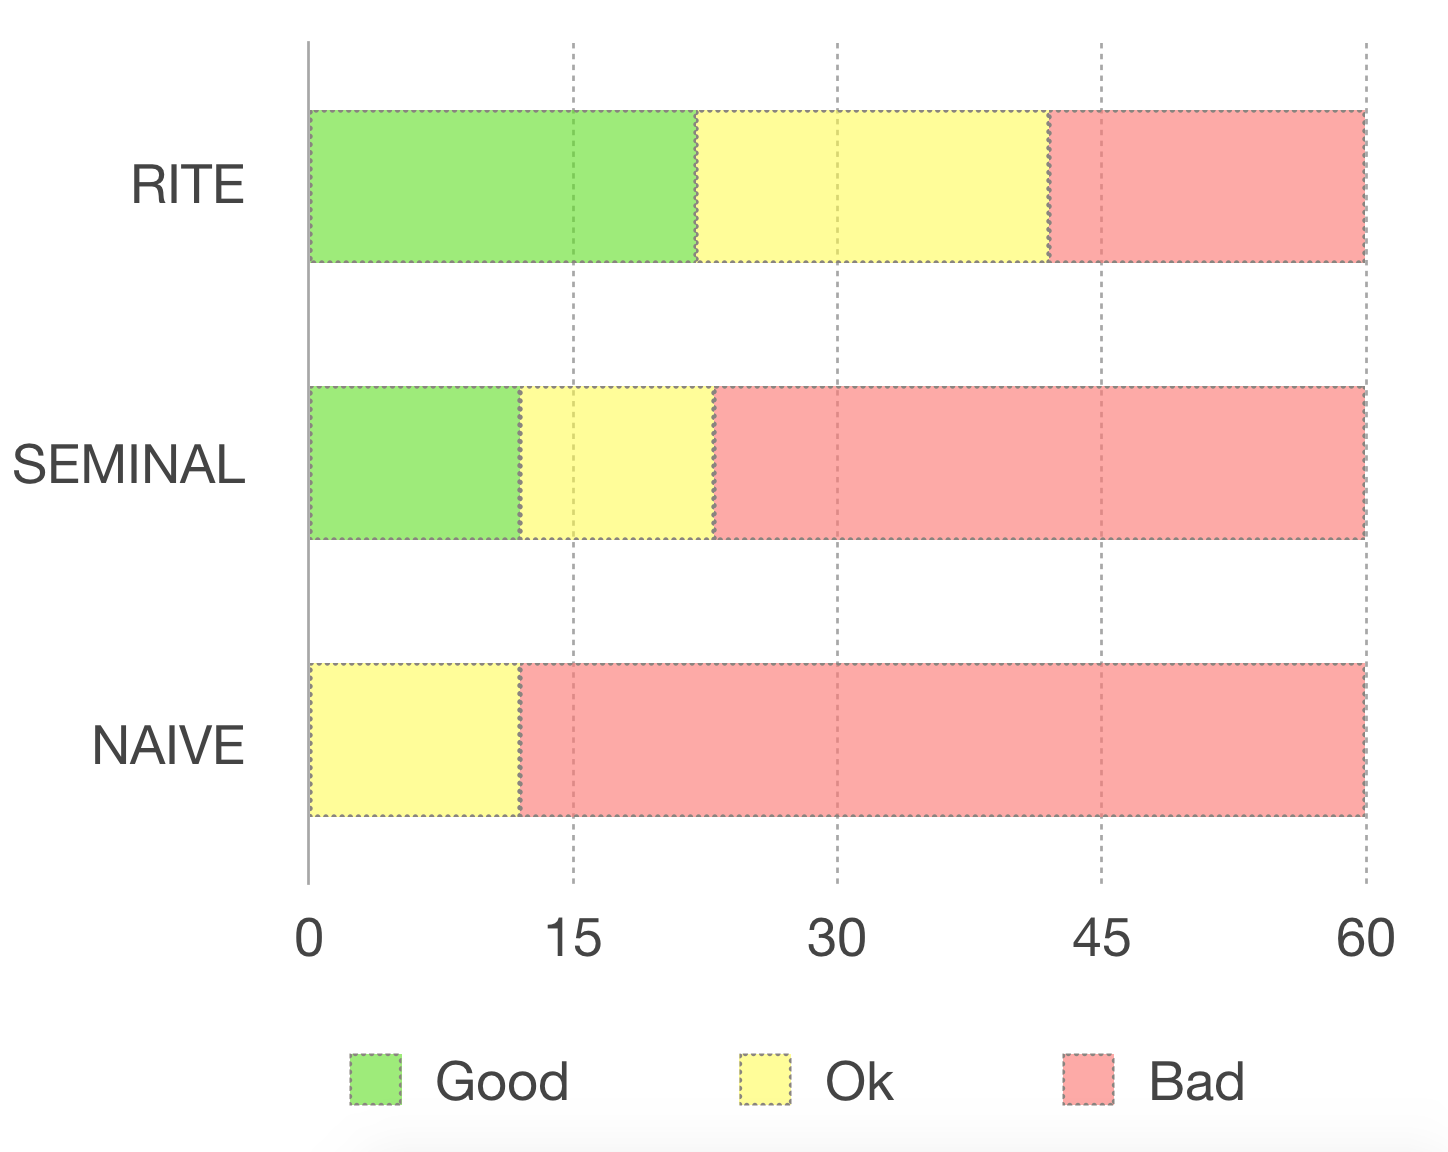
\includegraphics[height=1.5in]{comparison.png}
  \caption{Rating the errors generated by \toolname, \seminal and \naive enumeration.}
  \label{fig:comparison}
\end{figure}

\section{Related Work}
\label{sec:related-work}

\paragraph{Error Localization.}

\paragraph{Fixing Type-Errors.}

\section{Conclusion}
\label{sec:conclusion}

We have presented analytic program repair, a new data-driven 
approach to provide repairs as feedback for type errors.
%
Our approach is to use a dataset of ill-typed
programs and their fixed versions to learn a representative set of fix
templates, which, via multi-class classification allows us to 
accurately predict fix templates for new ill-typed programs. 
These templates guide the synthesis of program repairs in 
a tractable and precise manner.

We have implemented our approach in \toolname, and demonstrate,
using a corpus of 4,500 ill-typed \ocaml programs drawn from 
two instances of an introductory programming course, 
that \toolname makes accurate fix predictions 69\% 
of the time when considering the top three templates 
and surpass 80\% when we consider the top six,
and that the predicted templates let us synthesize 
repairs for over 70\% of the test set in under 20 sec.
%
Finally, we conducted a user study with 29 participants 
which showed that \toolname's repairs are of higher 
quality than those from the state-of-the-art \seminal 
tool which incorporates several expert-guided heuristics 
for improving the quality of repairs and error messages.
%
Thus, our results demonstrate the unreasonable effectiveness
of data for generating better error messages.



%% Acknowledgments
\begin{acks}                            %% acks environment is optional
                                        %% contents suppressed with 'anonymous'
  %% Commands \grantsponsor{<sponsorID>}{<name>}{<url>} and
  %% \grantnum[<url>]{<sponsorID>}{<number>} should be used to
  %% acknowledge financial support and will be used by metadata
  %% extraction tools.
  This material is based upon work supported by the
  \grantsponsor{GS100000001}{National Science
    Foundation}{http://dx.doi.org/10.13039/100000001} under Grant
  No.~\grantnum{GS100000001}{nnnnnnn} and Grant
  No.~\grantnum{GS100000001}{mmmmmmm}.  Any opinions, findings, and
  conclusions or recommendations expressed in this material are those
  of the author and do not necessarily reflect the views of the
  National Science Foundation.
\end{acks}


%% Bibliography
\bibliography{bibliography}


%% Appendix
% \appendix
% \section{Appendix}

% Text of appendix \ldots

\end{document}
